
\setcounter{chapter}{3}
\setcounter{section}{0}
\setcounter{table}{0}
\setcounter{figure}{0}
\chapter* {\begin{flushleft}
CHƯƠNG 3\\
\end{flushleft}LẬP TRÌNH ỨNG DỤNG CƠ SỞ DỮ LIỆU} 
\addcontentsline{toc}{chapter}{Chương 3. Lập trình ứng dụng cơ sở dữ liệu}
%\thispagestyle{fancy}
Chương này tập trung vào sử dụng thư viện JDBC (Java DataBase Connectivity) để kết nối và truy xuất vào các  sở dữ liệu. Nôi dung của chương bao gồm:
\begin{itemize}
	\item Trình bày được khái niệm về JDBC; Các thành phần JDBC; Phân loại JDBC; Cơ
	chế hoạt động JDBC,...
	\item Thực hiện được việc tải và cài đặt JDBC driver cho project
	\item Trình bày được các phương pháp kết nối CSDL với các hệ QT CSDL SQL Server,
	Ocracle, MySQL,…
	\item Thực hiện được việc kết nối và truy xuất cơ sở dữ liệu
	\item Thực hiện được việc xử lý kết xuất kết quả truy xuất CSDL.
	\item  Xây dựng được ứng dụng Quản lý CSDL
\end{itemize}


\section{Giới thiệu JDBC}
JDBC  là một thư viện chuẩn cho phép các ứng dụng Java kết nối với nhiều cơ sở dữ liệu được cài đặt trên các hệ quản trị cơ sở dữ liệu  như MS Access, SQL Server, Oracle, DB2,... JDBC hỗ trợ các chức năng như tạo một kết nối đến một cơ sở dữ liệu, tạo câu lệnh
SQL (Structured Query Language), thực thi câu lệnh SQL, xem và thay đổi dữ liệu.

\section{Các thành phần trong JDBC}
JDBC bao gồm các thành phần như  Hình \ref{hinh31}, trong đó:
\begin{itemize}
	\item JDBC API: là một API (Application Programming Interface) hoàn toàn dựa trên Java, giúp truy xuất cơ sở dữ liệu từ  Java.
	\item JDBC Diver Manager: một lớp (class) giúp kết nối giữa ứng dụng Java đến các JDBC Driver.
	\item JDBC Driver: là thành phần cho phép ứng dụng Java tương tác với các	cơ sở dữ liệu  khác nhau.
\end{itemize}

\begin{figure}[!ht]
	\centering
	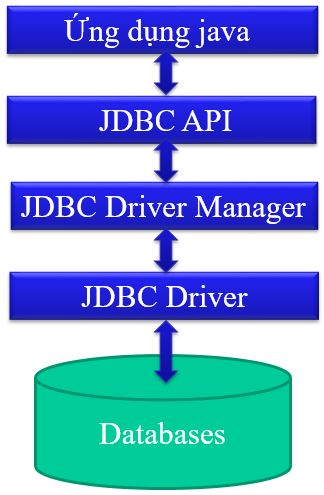
\includegraphics[scale=0.7]{Figures//Hinh31.jpg}
	\caption{ Các thành phần trong JDBC }\label{hinh31} 
\end{figure}
\section{Lược đồ lớp của JDBC}
\begin{figure}[!ht]
	\centering
	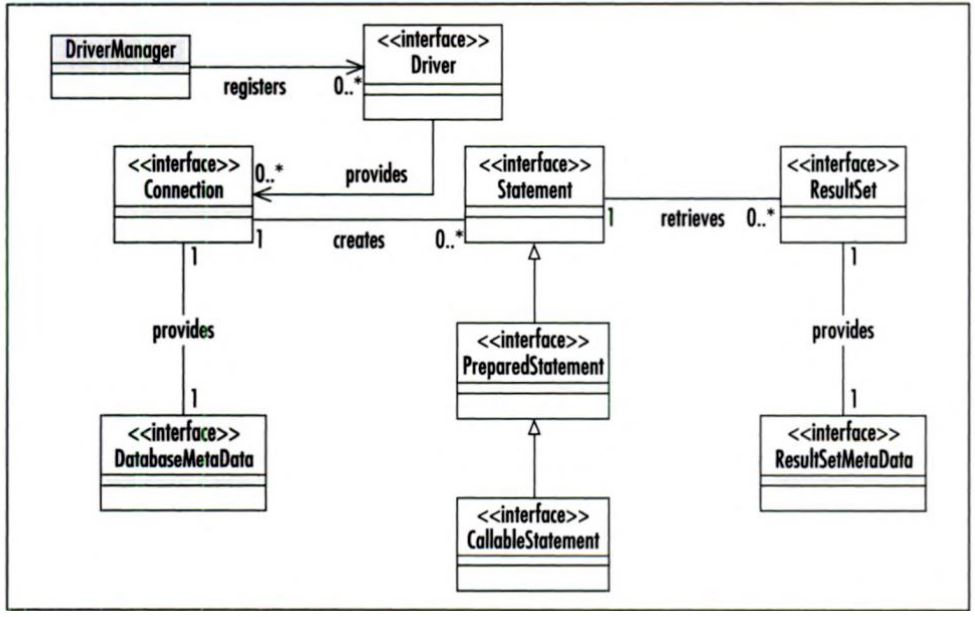
\includegraphics[scale=0.65]{Figures//Hinh32.jpg}
	\caption{ Các lớp và giao diện của JDBC }\label{hinh32} 
\end{figure}

JDBC bao gồm các lớp (class) và giao diện (interface) nằm trong gói java.sql.* như thể hiện ở Hình \ref{hinh32}, trong đó:
\begin{itemize}
	\item \textbf{Driver:} Giao diện này chứa các hàm trừu tượng để xử lý các kết nối đến cơ sở dữ liệu. Trong lập trình, chúng ta chủ yếu sử dụng lớp DriverManager được cài đặt từ giao diện Driver để quản lý các kết nối đến cơ sở được liệu.
	\item \textbf{DriverManager:} Lớp này quản lý một danh sách trình điều khiển cơ sở dữ liệu 	(database drivers).  Nó được dùng để nạp các Driver vào trong bộ nhớ và mở các kết nối tới một cơ sỡ dữ liệu nào đó.
	\item \textbf{Connection:} Đại diện cho một kết nối đến cơ sở dữ liệu. Được dùng để tạo ra các đối tượng Statement, PreparedStatement và CallableStatement.
	\item \textbf{Statement:} Đối tượng dùng để thực thi các câu lệnh SQL như câu lệnh thêm dữ liệu
	(insert), câu lệnh thay đổi dữ liệu (update), câu lệnh xoá dữ liệu (delete), câu lệnh
	xem dữ liệu (select), ...
	\item \textbf{PreparedSatement:} Giống như Statement nhưng có thể truyền tham số vào câu lệnh SQL.
	\item \textbf{CallableStatement:} được sử dụng để thực thi một thủ tục (Stored Procedure) được lưu trữ trong  hệ quản trị cơ sở dữ liệu.
	\item \textbf{ResultSet:} Đối tượng này sẽ quản lý dữ liệu sau khi chúng ta thực thi câu lệnh Select.  Một đối tượng ResultSet duy trì một con trỏ trỏ tới hàng dữ liệu hiện tại của nó, sử dụng con trỏ này để lấy dữ liệu từ các bảng (Tables) trong cơ sở dữ liệu.
	\item \textbf{DatabaseMetaData: }cung cấp các phương thức để lấy siêu dữ liệu (metadata) của cơ sở dữ liệu như tên sản phẩm cơ sở dữ liệu, phiên bản sản phẩm cơ sở dữ liệu, tên Driver, tên của các bảng, tên  view, ...
	\item \textbf{ResultSetMetaData:} cung cấp các phương thức để lấy siêu dữ liệu (metadata) của ResultSet như  tổng số cột, tên cột, kiểu của cột,...
\end{itemize}
Các bước truy xuất cơ sở dữ liệu
\begin{itemize}

\item \textbf{Bước 1:} Sử dụng lớp DirverManager để nạp trình điều khiển nhằm xác định hệ quản trị cơ sở dữ liệu cần sử dụng.
	\item \textbf{Bước 2:} Sử dụng lớp DirverManager  để tạo đường kết nối đến cơ sở dữ liệu. 
	\item \textbf{Bước 3:} Sử dụng đối tượng Connection để tạo ra các đối tượng Statement, PreparedStatement và CallableStatement.
	\item \textbf{Bước 4:}  Sử dụng các đối tượng Statement, PreparedStatement và CallableStatement để thực thi các câu lênh SQL hoặc thủ tục lưu trữ.
	\item \textbf{Bước 5:} Xử lý dữ liệu lấy về từ cơ sở dữ liệu
	\item  \textbf{Bước 6:} Giải phóng bộ nhớ và đóng kết nối

\end{itemize}
\section{Lớp DirverManager}
Lớp  DirverManager hoạt động như một giao diện giữa người dùng và các trình điều kiển (Driver). Nó theo dõi các trình điều khiển có sẵn và xử lý việc thiết lập kết nối giữa một cơ sở dữ liệu và trình điều khiển thích hợp. Lớp DriverManager duy trì một danh sách các trình điều khiển được đăng ký  bằng cách gọi phương thức DriverManager.registerDriver().

Để DriverManager nạp trình điều khiển thì trong project chúng ta phải thêm thư viện tương ứng với hệ quản trị cơ sở dữ liệu ta cần kết nối đến, Bảng \ref{bang31} liệt kê một số thư viện điều khiển thường dùng.
\begin{center}
	\begin{longtable}{|m{1cm}|m{3cm}|m{7cm}|}
		\caption[Một số thư viện điều khiển dùng trong JDBC]{Một số thư viện điều khiển dùng trong JDBC}
		\label{bang31}
		\endfirsthead
		\endhead
		\hline
		\multicolumn{1}{|c|}{\textbf{STT}} &\multicolumn{1}{c|}{	\textbf{ HQTCSDL}}
			&\multicolumn{1}{c|}{	\textbf{Tên thư viện điều khiển}}\\ \hline
	1&	MySQL & 	Mysql-connector-java-X.Y.Z.bin.jar (X.Y.Z là số hiệu của từng phiên bản) \\ \hline
	2&SQL Server &	sqljdbc.jar, sqljdbc4.jar \\ \hline
	3&	Oracle &	jodbc5.jar, jodbc6.jar, ... \\ \hline 
	4&	PostgreSQL &	Postgresql-9.1-902.jdbc4.jar \\ \hline 
	5&	SQLite &	Sqlite-jdbc-3.7.2.jar\\ \hline 
	\end{longtable}
\end{center}
\vspace{-1cm}
Ví dụ 3.4.1: Khi làm việc trên SQl Server, chúng ta cần thêm thư viện điều khiển sqljdbc4.rar vào Project  theo các bước:
\begin{itemize}
	\item Bước 1: Download thư viện điều  khiển sqljdbc4.rar về máy.
	\item Bước 2: Tạo 1 project trên Eclipse.
	\item Bước 3: Nhấn Alt + Enter, chọn Java Build Path, chọn Add External JARs như Hình \ref{hinh33}, sau đó chọn file  sqljdbc4.rar download ở Bước 1.

\end{itemize}
	\begin{figure}[!ht]
	\centering
	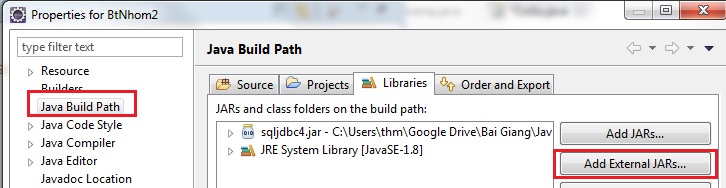
\includegraphics[scale=0.8]{Figures//Hinh33.jpg}
	\caption{ Thêm thư viện điều khiển vào Project của Eclipse }\label{hinh33} 
\end{figure}

\textbf{Một số phương thức thường dùng trong lớp DirverManager}


 \textbf{a. public static void registerDriver(Driver driver) throws SQLException}: 
	Phương thức này được sử dụng để đăng ký trình điều khiển đã cho với DriverManager.
	
	Ví dụ 3.4.2: cần đăng ký trình điều khiển để làm việc với SqlServer:
		\lstset{language=Java}
	\begin{lstlisting}[escapechar=`]
		Driver dr=new com.microsoft.sqlserver.jdbc.SQLServerDriver();
		DriverManager.registerDriver(dr);
	\end{lstlisting}
	
Ngoài cách trên, người ta thường dùng Class.forName()  để đăng ký trình điều khiển đây là hướng tiếp cận chung và được dùng phổ biến để đăng ký một Driver. Cú pháp:
	\lstset{language=Java}

\begin{lstlisting}[escapechar=`]
public static void Class.forName(String DatabaseDriver) throws ClassNotFoundException
\end{lstlisting}
Trong đó, DatabaseDriver là một chuỗi để xác đinh tên hệ quản trị cơ sỡ dữ liệu, Bảng \ref{bang32} trình bày một số DatabaseDriver thường dùng:
\begin{center}
	\begin{longtable}{|m{1cm}|m{2cm}|m{8cm}|}
		\caption[Một số DatabaseDriver thường dùng]{Một số DatabaseDriver thường dùng}
		\label{bang32}
		\endfirsthead
		\endhead
		\hline
		\multicolumn{1}{|c|}{\textbf{STT}} &\multicolumn{1}{c|}{	\textbf{ HQTCSDL}}
		&\multicolumn{1}{c|}{	\textbf{DatabaseDriver}}\\ \hline
		1&	MySQL & com.mysql.jdbc.Driver \\ \hline
		2&SQL Server &	com.microsoft.sqlserver.jdbc.SQLServerDriver \\ \hline
		3&	Oracle &	oracle.jdbc.driver.OracleDriver\\ \hline 
		4&	PostgreSQL &	org.postgresql.Driver \\ \hline 
		5&	Microsoft Access
		 &	sun.jdbc.odbc.JdbcOdbcDriver
		\\ \hline 
	\end{longtable}
\end{center}
\vspace{-1cm}
Ví dụ 3.4.3: 

Đăng ký trình điều khiển để làm việc với SqlServer
	\lstset{language=Java}
	\begin{lstlisting}[escapechar=`]
Class.forName("com.microsoft.sqlserver.jdbc.SQLServerDriver");
	\end{lstlisting}

 Đăng ký trình điều khiển để làm việc với MySql
\lstset{language=Java}
\begin{lstlisting}[escapechar=`]
Class.forName("com.mysql.jdbc.Driver");
\end{lstlisting}

\textbf{2. public static void deregisterDriver(Driver driver)}

Phương thức này được sử dụng để xóa Driver đã cho khỏi danh sách đăng ký với DriverManager.

Ví dụ 3.4.4: Đăng ký trình điều khiển để làm việc với SqlServer, sau đó xóa trình điều khiển ra khỏi danh sách:

\lstset{language=Java}
\begin{lstlisting}[escapechar=`]
Driver dr=new com.microsoft.sqlserver.jdbc.SQLServerDriver();
DriverManager.registerDriver(dr);
DriverManager.deregisterDriver(dr);
\end{lstlisting}
\textbf{3. public static Connection getConnection(String DatabaseURL)}

Phương thức này được sử dụng để thiết lập kết nối đến cơ sở dữ liệu, các thông tin kết nối được lưu trong DatabaseURL. DatabaseURL là một chuỗi thường lưu tên Server chứa hệ quản trị cơ sở dữ liệu, tên cơ sở dữ liệu cần kết nối. Một số DatabaseURL có thể lưu  username và password để truy cập vào cơ sở dữ liệu. Một số DatabaseURL thường dùng được lưu ở Bảng \ref{bang33}.


\begin{center}
	\begin{longtable}{|m{1cm}|m{2cm}|m{8cm}|}
		\caption[Một số DatabaseURL thường dùng]{Một số DatabaseDriver thường dùng}
		\label{bang33}
		\endfirsthead
		\endhead
		\hline
		\multicolumn{1}{|c|}{\textbf{STT}} &\multicolumn{1}{c|}{	\textbf{ HQTCSDL}}
		&\multicolumn{1}{c|}{	\textbf{DatabaseDriver}}\\ \hline
		1&	MySQL & jdbc:mysql://<Tên Server>:<port>/<Tên CSDL>\\ \hline
		2&SQL Server &	jdbc:sqlserver://<Tên server>:<port>; databaseName=<Tên CSDL>;user=…; password=… 
		 \\ \hline
		3&	Oracle & jdbc:oracle:thin:@<Tên server>:<port>: <Tên CSDL>
		\\ \hline 
		4&	PostgreSQL &jdbc:postgresql://<Tên server>:<port>/<Tên CSDL>\\ \hline 
		5&	Microsoft Access
		&	jdbc:odbc:Driver={Microsoft Access Driver (*.mdb)};
		DBQ=<Tên CSDL.mdb>
		\\ \hline 
	\end{longtable}
\end{center}
\vspace{-1cm}
Ví dụ 3.4.5: Viết chương trình kết nối đến CSDL: QlNv của SQLServer; Tên Server: ADMIN; Username: sa; password:123
 \lstset{language=Java,
 tabsize = 4, %% set tab space width
 showstringspaces = false, %% prevent space marking in strings, string is defined as the text that is generally printed directly to the console
 numbers = left, %% display line numbers on the left
 commentstyle = \color{green}, %% set comment color
 keywordstyle = \color{blue}, %% set keyword color
 stringstyle = \color{red}, %% set string color
 rulecolor = \color{black}, %% set frame color to avoid being affected by text color
 basicstyle = \small \ttfamily , %% set listing font and size
 breaklines = true, %% enable line breaking
 numberstyle = \tiny,}
 \begin{lstlisting}[escapechar=`]
import java.sql.*;
public class ViDu345 {
public static void main(String[] args) {
	try {
		//b1 `Nạp trình điều khiển`
		String driver= "com.microsoft.sqlserver.jdbc.SQLServerDriver";
		Class.forName(driver);
		//b2: `Kết nối vào CSDL`
		String urlDatabase ="jdbc:sqlserver://ADMIN:1433; databaseName=QlNv; user=sa; password=123";
		Connection   cn=DriverManager.getConnection(urlDatabase);
		System.out.println("Da ket noi");
	} catch (Exception e) {
		e.printStackTrace();
	}
  }
}
 \end{lstlisting}
 Khi chạy chương trình trên, một số lỗi thường gặp:
 
 \textbf{a. Chưa thêm thư viện  sqljdbc4 vào Project:}
Khi chưa thêm thư viện sqljdbc4.rar vào Project sẽ hiển thị lỗi như Hình \ref{hinh33_1}. Để khắc phục lỗi này ta thực hiện 3 bước như Ví dụ 3.4.1.
  	\begin{figure}[!ht]
  	\centering
  	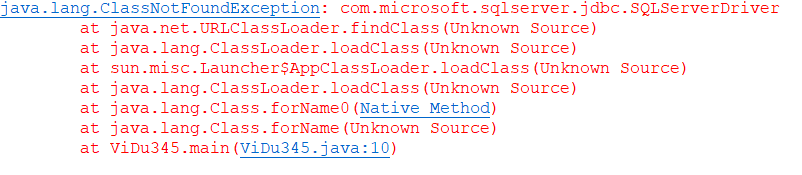
\includegraphics[scale=0.6]{Figures//Hinh33_1.png}
  	\caption{ Lỗi chưa thêm thư viện vào Project  }\label{hinh33_1} 
  \end{figure}

 \textbf{b. Chưa bật giao thức TCP và mở cổng trong SQLServer:} Trong một số phiên bản của SQLServer khi cài lên sẽ chưa mở giao thức TCP và cổng 1433. Vì vậy, khi chạy  chương trình sẽ báo lỗi như Hình \ref{hinh33_2}.
 
	\begin{figure}[ht]
	\centering
	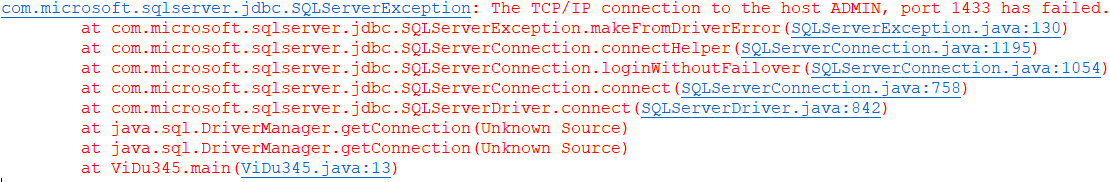
\includegraphics[scale=0.55]{Figures//Hinh33_2.png}
	\caption{ Lỗi chưa mở cổng và bật giao thức TCP  }\label{hinh33_2} 
	\end{figure}
Để khắc phục lỗi này ta thực hiện theo các bước sau:

   \textbf{Bước 1:} Nhấn Start và đi tìm và mở SQL Server Configuration Manager như Hình \ref{hinh33_3}.  Chọn SQL Server Network Configuration, chọn Protocols for ... và kích đôi lên TCP/IP.
   	\begin{figure}[ht]
   	\centering
   	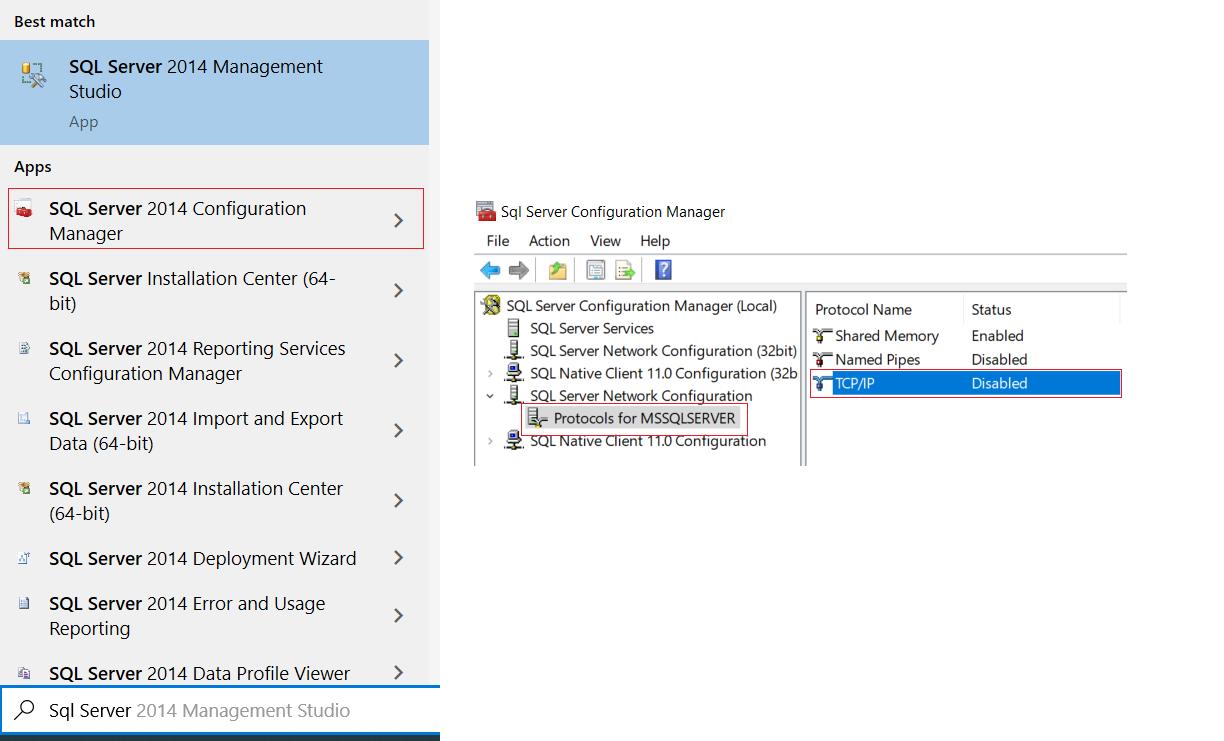
\includegraphics[scale=0.5]{Figures//Hinh33_3.png}
   	\caption{ Mở SQL Server Configuration Manager  }\label{hinh33_3} 
   \end{figure}

   \textbf{Bước 2:} Bật giao thức TCP và mở cổng 1433 như Hình \ref{hinh33_4}
  	\begin{figure}[!ht]
	\centering
	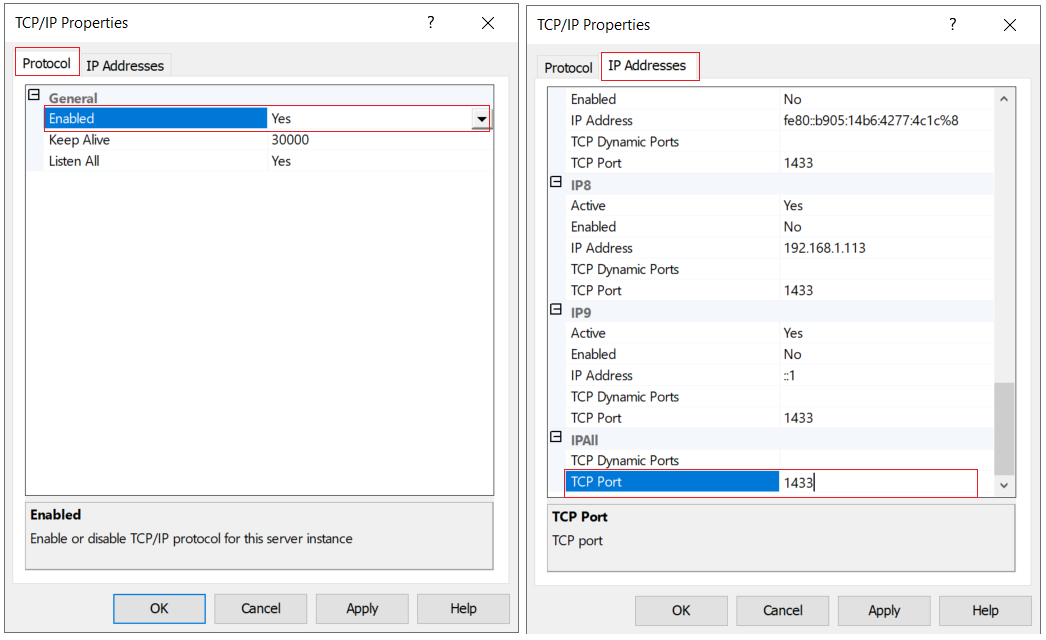
\includegraphics[scale=0.5]{Figures//Hinh33_4.png}
	\caption{ Bật giao thức TCP và mở cổng 1433 }\label{hinh33_4} 
\end{figure}

\textbf{Bước 3:} Tắt và khởi động lại dịch vụ của SQL Server như Hình \ref{hinh33_5}. Kích phải lên dịch vụ của SQL Server chọn Stop để tắt dịch vụ, sau đó  kích phải lên dịch vụ của SQL Server chọn Start để khởi động lại dịch vụ.
\begin{figure}[!ht]
	\centering
	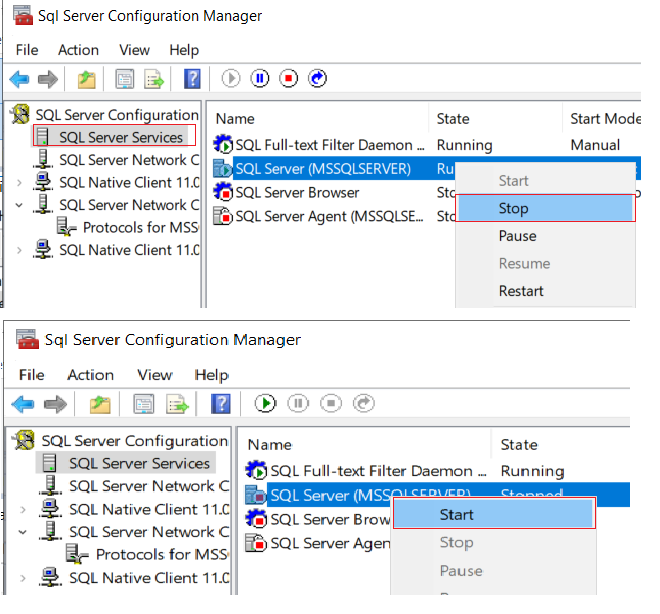
\includegraphics[scale=0.6]{Figures//Hinh33_5.png}
	\caption{ Tắt và khởi động lại dịch vụ của SQL Server}\label{hinh33_5} 
\end{figure}

 \textbf{c. Chưa bật cấu hình user và password để login vào SQL Server:} Trong quá trình cài SQLServer ta chưa cấu hình tài khoản để login vào SQL Server. Vì vậy, khi chạy  chương trình sẽ báo lỗi như Hình \ref{hinh33_6}.
 
 	\begin{figure}[!ht]
 	\centering
 	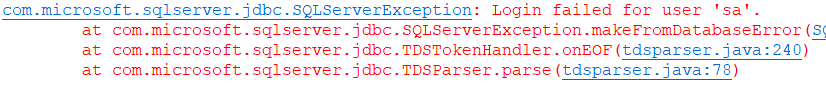
\includegraphics[scale=0.7]{Figures//Hinh33_6.png}
 	\caption{ Chưa cấu hình tài khoản để login vào SQL Server  }\label{hinh33_6} 
 \end{figure}

Để khắc phục lỗi này ta lần lượt thực hiện theo các bước để cấu hình user và password như sau:

\textbf{Bước 1:} Khởi động SQL Server Management Studio và đăng nhập vào theo tài khoản của Window như Hình \ref{hinh33_7}
	\begin{figure}[!ht]
	\centering
	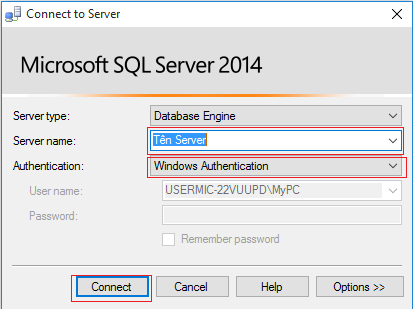
\includegraphics[scale=0.7]{Figures//Hinh33_7.png}
	\caption{Đăng nhập vào SQL Server  }\label{hinh33_7} 
  \end{figure}

\textbf{Bước 2:} Cấu hình để người dùng đăng nhập bằng tài khoản trong SQL Server như Hình \ref{hinh33_8}. Kích phải lên Tên Server, chọn Properties, tại Security chọn SQL Server and Window Authentication mode.  

\begin{figure}[!ht]
	\centering
	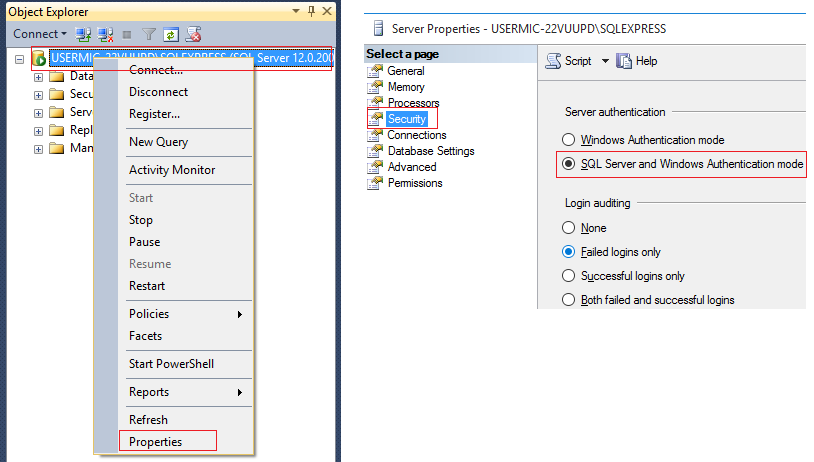
\includegraphics[scale=0.6]{Figures//Hinh33_8.png}
	\caption{Cấu hình để người dùng đăng nhập bằng tài khoản  }\label{hinh33_8} 
\end{figure}
 
\textbf{Bước 3:} Đặt mật khẩu và cho phép user: sa đăng nhập vào SQL Server như Hình  \ref{hinh33_9}. Kích phải lên user: sa, chọn Properties, Chọn General, sau đó nhập mật khẩu và nhập lại mật khẩu. Chọn Status và chọn Enabled để cho phép tài khoản sa đăng nhập vào hệ thống.  
\textbf{Bước 4:} Tắt và mở lại dịch vụ SQL Server. Kích phải lên Tên Server chọn Stop, sau đó  kích phải lên Tên Server chọn Start.
\begin{figure}[!ht]
	\centering
	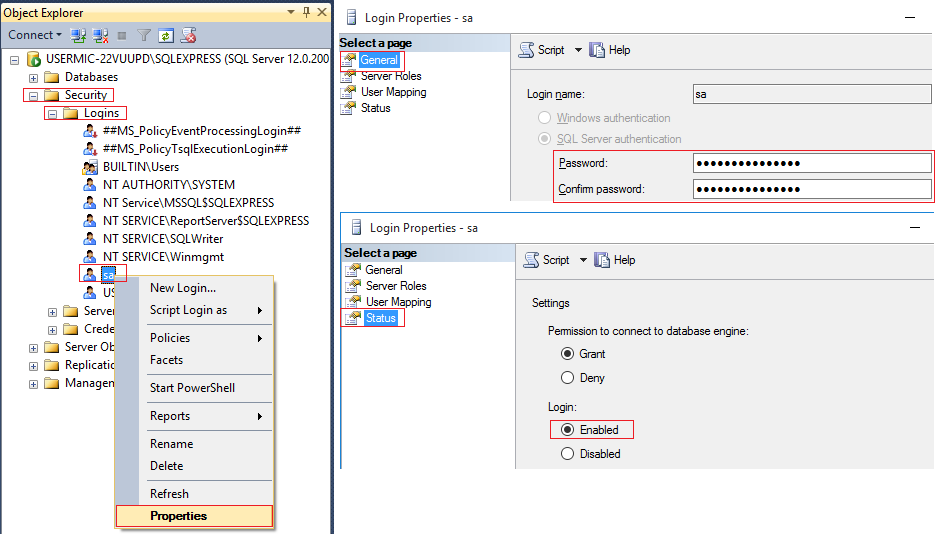
\includegraphics[scale=0.5]{Figures//Hinh33_9.png}
	\caption{Đặt mật khẩu và cho phép user: sa đăng nhập  }\label{hinh33_9} 
\end{figure}

\textbf{4. public static Connection getConnection(String url,String userName,String password)}

Trong trường hợp một số DatabaseURL không chứa username, và password thì dùng phương thức này để thiết lập kết nối đến CSDL.

Ví dụ 3.4.6. Viết chương trình kết nối đến CSDL: QlNv của MySql; Tên Server: ADMIN; Username: root; password:123
 \lstset{language=Java,
 tabsize = 4, %% set tab space width
 showstringspaces = false, %% prevent space marking in strings, string is defined as the text that is generally printed directly to the console
 numbers = left, %% display line numbers on the left
 commentstyle = \color{green}, %% set comment color
 keywordstyle = \color{blue}, %% set keyword color
 stringstyle = \color{red}, %% set string color
 rulecolor = \color{black}, %% set frame color to avoid being affected by text color
 basicstyle = \small \ttfamily , %% set listing font and size
 breaklines = true, %% enable line breaking
 numberstyle = \tiny,}
\begin{lstlisting}[escapechar=`]
import java.sql.Connection;
import java.sql.DriverManager;
public class ViDu346 {
public static void main(String[] args) {
	try {
		//b1 `Nạp trình điều khiển`
		String driver="com.mysql.jdbc.Driver";
		Class.forName(driver);
		//b2: `Kết nối vào CSDL`
		String urlDatabase ="jdbc:mysql://localhost/QlNv";
		Connection   cn=DriverManager.getConnection( urlDatabase,"root","123");
		System.out.println("Da ket noi");
	} catch (Exception e) {
	e.printStackTrace();
	}
 }
}
\end{lstlisting}

Sau khi kết nối vào CSDL thì phương thức getConnection sẽ trả về một đối tượng Connection, sử dụng đối tượng Connection để tạo ra  các đối tượng Statement, PreparedStatement và CallableStatement.\\
\textbf{5. public static void setLoginTimeout(int second)}

Phương thức này thiết lập thời gian (bằng giây) tối đa mà một Driver sẽ đợi trong khi cố gắng kết nối với một CSDL.\\
\textbf{6. public static int getLoginTimeout()}

Phương thức này lấy thời gian (bằng giây) tối đa mà một Driver sẽ đợi trong khi cố gắng truy cập vào một CSDL.
\section{Đối tượng Connection}
Sau khi đã nạp trình điều khiển để xác định hệ quản trị cơ sở dữ liệu và đã kết nối vào cơ sở dữ liệu, bước tiếp theo chúng ta cần  lấy dữ liệu về để xử lý và lưu lại dữ liệu vào cơ sở dữ liệu. Để thực hiện được các việc này, chúng ta sử dụng các phương thức của Connection, một số phương thức của Connection:\\ 
\textbf{1. public Statement createStatement()}

Phương thức này tạo đối tượng Statement để thực thi các truy vấn SQL. Khi lấy dữ liệu từ cơ sở dữ liệu về chúng ta chỉ duyệt các bản ghi từ trên xuống, không thể di chuyển con trỏ đến bản ghi bất kỳ và không thể cập nhật lại dữ liệu.\\
\textbf{2. public Statement createStatement(int resultSetType,int resultSetConcurrency) throws SQLException}

Phương thức này cũng tạo ra một đối tượng Statement khắc phục các nhược điểm của của phương thức createStatement(), với phương thức reateStatement(int resultSetType,int resultSetConcurrency) ta có thể di chuyển con trỏ đến vị trí bất kỳ, cho phép người dùng cập nhật lại dữ liệu trên các bản ghi được lấy về, trong đó:

resultsetType là 1 trong 3 kiểu:
\begin{itemize}
	\item ResultSet.TYPE \text{\_}FORWARD \text{\_}ONLY: chỉ di chuyển con trỏ đi tới.
	\item ResultSet.TYPE \text{\_}SCROLL \text{\_}INSENSITIVE: cho phép di chuyển con trỏ nhưng không cho phép cập nhật lại dữ liệu
	\item ResultSet.TYPE \text{\_}SCROLL \text{\_}SENSITIVE: cho phép di chuyển con trỏ và cho phép cập nhật lai dữ liệu.
\end{itemize}

resultSetConcurrency là 1 trong 2 kiểu:
\begin{itemize}
	\item ResultSet.CONCUR \text{\_}READ \text{\_}ONLY: dữ liệu lấy về chỉ đọc không thể cập nhật được.
	
	\item ResultSet.CONCUR \text{\_}UPDATABLE: Cho phép cập nhật lại dữ liệu.
\end{itemize}

\textbf{3. public PreparedStatement prepareStatement(String sql) throws SQLException}
Trong đó: chuỗi sql chứa câu lệnh SQL.

Giống như phương thức Statement() nó được dùng để thực thi truy vấn SQL nhưng có thể sử dụng tham số trong câu lênh SQL. Thực tế, ta nên dùng phương này ngay cả khi không cần phải truyền tham số bởi nó thực thi nhanh hơn do được nạp trước (preload) khi thực thi. PreparedStatement được kế thừa từ Statement, vì vậy mọi phương thức của Statement đều có thể dùng ở đây.  

\textbf{4. public PreparedStatement prepareStatement(String sql, int resultSetType, int resultSetConcurrency)throws SQLException}

Phương thức này và các tham số của nó giống như phương thức createStatement(int resultSetType,int resultSetConcurrency) như ta có thể truyền tham số vào câu lệnh sql.

Ví dụ 3.4.7. Đã có cơ sở dữ liệu QlNv trong SqlServer, trong cơ sở dữ liệu này đã có bảng DonVi(\textbf{\underline{MaDonVi}}, TenDonVi), đoạn mã dưới đây sử dụng phương thức prepareStatement để tạo ra một câu lệnh SQL với các tham số nhằm mục đích chuẩn bị thêm vào  1 đơn vị vào bảng DonVi.
 \lstset{language=Java,
 tabsize = 4, %% set tab space width
 showstringspaces = false, %% prevent space marking in strings, string is defined as the text that is generally printed directly to the console
 numbers = left, %% display line numbers on the left
 commentstyle = \color{green}, %% set comment color
 keywordstyle = \color{blue}, %% set keyword color
 stringstyle = \color{red}, %% set string color
 rulecolor = \color{black}, %% set frame color to avoid being affected by text color
 basicstyle = \small \ttfamily , %% set listing font and size
 breaklines = true, %% enable line breaking
 numberstyle = \tiny,}
\begin{lstlisting}[escapechar=`]
import java.sql.Connection;
import java.sql.DriverManager;
import java.sql.PreparedStatement;
public class ViDu347 {
public static void main(String[] args) {
	try { 
		//b1 `Nạp trình điều khiển`
		String driver= "com.microsoft.sqlserver.jdbc.SQLServerDriver";
		Class.forName(driver);
		//b2: `Kết nối vào CSDL`
		String urlDatabase ="jdbc:sqlserver://ADMIN:1433; databaseName=Qlnv;user=sa;password=123";
		Connection   cn=DriverManager.getConnection(urlDatabase);
		//b3: `Tạo câu lệnh PreparedStatement`
		String sql="insert into DonVi values (?,?)";
		PreparedStatement cmd=cn.prepareStatement(sql);
	} catch (Exception e) {
		e.printStackTrace();
	}
 }
}

\end{lstlisting}


\textbf{5. public CallableStatement prepareCall("{ call tên\_thủ\_tục( các tham số của thủ tục)}");}

Được sử dụng để thực thi một thủ tục lưu trữ (Stored Procedure) trong SQL Server. Ta có thể sử dụng dấu ? để truyền vào các tham số của thủ tục. CallableStatement được thừa kế từ PreparedStatement.
  
\textbf{5. public void setAutoCommit(boolean autoCommit) throws SQLException
}

Phương thức này thiết lập Connection trong chế độ auto-commit. Nếu một Connection trong chế độ tự động ký thác thì tất cả các lệnh SQL của nó sẽ được thực thi và ký thác sau mỗi giao tác. Nếu tham số autoCommit được thiết lập là true tức là kích hoạt chế độ auto-commit, nếu là false là vô hiệu hóa chế độ này.

\textbf{6. public void commit() throws SQLException}

Phương thức này lưu các thay đổi đã được thực hiện trước đó. Phương thức này nên chỉ được sử dụng khi chế độ auto-commit đã bị vô hiệu hóa.

\textbf{7. public void rollback()}

Phương thức này xóa tất cả các thay đổi đã được thực hiện trước đó và quay về trạng thái trước khi thực hiện thay đổi. Phương thức này nên chỉ được sử dụng khi chế độ auto-commit đã bị vô hiệu hóa.

\textbf{8. public void close()}

Phương thức này đóng kết nối và giải phóng tài nguyên.

Ví dụ 3.4.8. Ví dụ này trình bày các bước để quyết định thực hiện các công việc hoặc phục hồi lại các công việc nếu chương trình bị lỗi.

\lstset{language=Java,
tabsize = 4, %% set tab space width
showstringspaces = false, %% prevent space marking in strings, string is defined as the text that is generally printed directly to the console
numbers = left, %% display line numbers on the left
commentstyle = \color{green}, %% set comment color
keywordstyle = \color{blue}, %% set keyword color
stringstyle = \color{red}, %% set string color
rulecolor = \color{black}, %% set frame color to avoid being affected by text color
basicstyle = \small \ttfamily , %% set listing font and size
breaklines = true, %% enable line breaking
numberstyle = \tiny,}
\begin{lstlisting}[escapechar=`]
import java.sql.Connection;
import java.sql.DriverManager;
import java.sql.PreparedStatement;
public class ViDu348 {
public static void main(String[] args) {
	Connection   cn=null;
	try { 
		//b1 `Nạp trình điều khiển`
		String driver= "com.microsoft.sqlserver.jdbc.SQLServerDriver";
		Class.forName(driver);
		//b2: `Kết nối vào CSDL Qlnv, tên Server: ADMIN, user:sa, password=123`
		String urlDatabase ="jdbc:sqlserver://ADMIN:1433; databaseName=Qlnv;user=sa; password=123";
		cn=DriverManager.getConnection(urlDatabase);
	    //b3: `Đặt chế độ AutoCommi=false`
		cn.setAutoCommit(false);
		//b4: `Thực thi các công việc như thêm, xóa, cập nhật vào cơ sở dữ liệu`
		  `...`
		//b5: `Quyết định thực thi các công việc ở B4`
		cn.commit();
		cn.close();`//Đóng kết nối`
		System.out.println("`Đã hoàn thành các công việc`");
	} catch (Exception e) {
		System.out.print("`Chương trình bị lỗi`");
		try { 
			//b6:` Phục hồi lại công việc ở ở B4`
			cn.rollback();
			cn.close();`//Đóng kết nối`
		} catch (Exception e2) {
		System.out.print("`Không thể phục hồi`");
	}
  }
 }
}
\end{lstlisting}

Ví dụ 3.4.9.\label{3.4.9} Để đơn giản B1 và B2 ta viết một lớp DungChung và xây dựng một hàm tĩnh để kết nối và trả về đường kết nối đến cơ sở dữ liệu Qlnv trên máy chủ ADMIN với user và password để login vào CSDL là: sa và 123. 

\lstset{language=Java,
	tabsize = 4, %% set tab space width
	showstringspaces = false, %% prevent space marking in strings, string is defined as the text that is generally printed directly to the console
	numbers = left, %% display line numbers on the left
	commentstyle = \color{green}, %% set comment color
	keywordstyle = \color{blue}, %% set keyword color
	stringstyle = \color{red}, %% set string color
	rulecolor = \color{black}, %% set frame color to avoid being affected by text color
	basicstyle = \small \ttfamily , %% set listing font and size
	breaklines = true, %% enable line breaking
	numberstyle = \tiny,}
\begin{lstlisting}[escapechar=`]
import java.sql.Connection;
import java.sql.DriverManager;
public class DungChung {
   public static Connection KetNoi() throws Exception{
	//b1 `Nạp trình điều khiển`
   String driver="com.microsoft.sqlserver.jdbc.SQLServerDriver";
   Class.forName(driver);
	//b2: `Kết nối vào CSDL Qlnv, tên Server: ADMIN, user:sa, password=123`
   String urlDatabase ="jdbc:sqlserver://ADMIN:1433; databaseName=Qlnv;user=sa; password=123";
   return DriverManager.getConnection(urlDatabase);
 }
}
\end{lstlisting}


\section{Đối tượng Statement}
Statment được tạo ra bởi đối tượng Connection dùng để thực thi các câu lệnh SQL, một số phương thức thường dùng:

\textbf{1. public ResultSet executeQuery(String sql)}

Thực thi một lệnh SQL đã cho và trả về một đối tượng Resultset. Tham số sql là một chuỗi chứa câu lệnh SQL: SELECT. 


\textbf{2. public int executeUpdate(String sql)}

Thực thi lệnh sql đã cho, câu lệnh sql có thể là INSERT, UPDATE, DELETE hoặc một lệnh SQL mà không trả về giá trị  như lệnh SQL về định nghĩa dữ liệu: CREATE TABLE, CREATE DATABASE, ... 

Phương thức trả về số mẫu tin có hiệu lực, ví dụ trả về số mẫu tin thêm được hoặc xóa được hoặc cập nhật được. Nếu câu lệnh SQL chứa các câu lệnh SQL về định nghĩa dữ liệu hàm sẽ trả về bằng 0.

Ví dụ 3.6.1: Chèn thêm 1 dòng vào bảng DonVi có cấu trúc như ví dụ 3.4.7. Đoạn mã sau chưa kiểm tra trùng MaDonVi.
\lstset{language=Java,
	tabsize = 4, %% set tab space width
	showstringspaces = false, %% prevent space marking in strings, string is defined as the text that is generally printed directly to the console
	numbers = left, %% display line numbers on the left
	commentstyle = \color{green}, %% set comment color
	keywordstyle = \color{blue}, %% set keyword color
	stringstyle = \color{red}, %% set string color
	rulecolor = \color{black}, %% set frame color to avoid being affected by text color
	basicstyle = \small \ttfamily , %% set listing font and size
	breaklines = true, %% enable line breaking
	numberstyle = \tiny,
}
\begin{lstlisting}[escapechar=`]
import java.sql.*;
public class ViDu361 {
public static void main(String[] args) {
Connection   cn=null;
try { 
	//b1, b2
	cn=DungChung.KetNoi();
	//b3: `Đặt chế độ AutoCommi=false`
	cn.setAutoCommit(false);
	//b4: `Thêm vào bảng đơn vị 1 bản ghi với mã đơn vị là cntt và tên đơn vị là Công nghệ thông tin`
	String madv="cntt";
	String tendv="`Công nghệ thông tin`";
	//`Thiết lập câu lệnh sql`
	String sql="insert into DonVi values ('" +madv+"',N'"+ tendv+"')";
	Statement cmd=cn.createStatement();
	int smt=cmd.executeUpdate(sql);
	System.out.print("`Số mẫu tin thêm được:` "+ smt);
	//b5: `như trong ví dụ 3.4.8`
	`...`
} catch (Exception e) {
	System.out.print("`Chương trình bị lỗi`");
	try { 
		//b6: `Phục hồi lại công việc ở ở B4`
		cn.rollback();
		cn.close();//`Đóng kết nối`
	} catch (Exception e2) {
		System.out.print("`Không thể phục hồi`");
	}
  }
 }
}
\end{lstlisting}

\textbf{\underline{Chú ý:}} Theo ví dụ trên nếu Tendv="Baker's Chocolate" thì câu lệnh SQL sẽ bị lỗi cú pháp vì sau khi ghép câu lệnh sql sẽ là "insert into DonVi values (\textbf{'}cntt\textbf{'},N\textbf{'}Baker\textbf{'}s Chocolate\textbf{'}). Để khắc phục nhược điểm này ta dùng đối tượng PreparedStatement thay vì dùng đối tượng Statement.

\textbf{3. void close() throws SQLException}

Phương thức được sử dụng để đóng đối tượng Statement và giải phóng tài nguyên ngay lập tức. Khi đã đóng đối tượng Statement rồi, thì các lời gọi phương thức nào tới đối tượng đó sẽ không hoạt động. Khi một đối tượng Statement đã bị đóng thì đối tượng ResultSet của nó cũng bị đóng theo.

\section{Hạn chế của đối tượng Statement}
Khi sử dụng đối tượng Statement, thường nối (ghép) các chuỗi lại với nhau để thiết lập câu lệnh SQL. 

Ví dụ 3.7.1: Để tìm kiếm một đơn vị trong bảng DonVi thì câu lệnh SQL là "Select * from DonVi where TenDonVi=N'"+\textbf{tendv}+"'", trong đó \textbf{tendv} do người dùng nhập vào.

Giả sử người dùng nhập \textbf{tendv=Công nghệ thông tin} thì sẽ tìm ra các đơn vị có tên là Công nghệ thông tin. Nhưng nếu người dùng nhập vào \textbf{ tendv=Baker's Chocolate }thì câu lệnh SQL sẽ bị sai cú pháp vì bị dư dấu ' trong câu lệnh SQL.

Ví dụ 3.7.2: Giả sử đã có bảng Login(\textbf{\underline{username}}, password) để người dùng đăng nhập vào hệ thống. Câu lệnh SQL để kiểm tra người dùng đăng nhập thành công hay không là: 
"select * from Login where username ='"+\textbf{un}+ "' and password='"+\textbf{pass}+"'", trong đó \textbf{un} và \textbf{pass} do người dùng nhập vào. Như vậy nếu người dùng nhập vào \textbf{un=nhập bất kỳ} và  \textbf{ pass= nhập bất kỳ' or '1'='1 } khi đó điều kiện của câu lệnh SQL  luôn đúng: select * from Login where username ='nhập bất kỳ' and password='nhập bất kỳ'\textbf{ or '1'=1'}". Điều này có nghĩa là cho dù người dùng không có tài khoản để đăng nhập họ vẫn đăng nhập thành công vào hệ thống. Đây được gọi là SQL Injection:

\textit{SQL injection là một kỹ thuật cho phép những kẻ tấn công lợi dụng lỗ hổng của việc kiểm tra dữ liệu đầu vào trong các ứng dụng  và các thông báo lỗi của hệ quản trị cơ sở dữ liệu trả về để inject (tiêm vào) và thi hành các câu lệnh SQL bất hợp pháp. SQL injection có thể cho phép những kẻ tấn công thực hiện các thao tác, delete, insert, update, v.v. trên cơ sở dữ liệu của ứng dụng, thậm chí là server mà ứng dụng đó đang chạy. SQL injection thường được biết đến như là một vật trung gian tấn công trên các ứng dụng  có dữ liệu được quản lý bằng các hệ quản trị cơ sở dữ liệu như SQL Server, MySQL, Oracle, DB2, Sysbase…}

Qua hai ví dụ trên ta thấy được các tác hại và hạn chế khi sử dụng Statement. Statement không có tham số hóa ? nên muốn truyền vào tham số chúng ta cần thêm dấu + để nối các chuỗi lại với nhau. Từ đó hacker hay người dùng xấu có thể cố tình truy cập vào hệ thống.

Vì vậy PreparedStatement sinh ra để khắc phục nhược điểm trên, PreparedStatement không nối chuỗi và dùng các tham số ? để truyền vào câu lệnh SQL, ví dụ:

String sql = "SELECT * FROM users WHERE username = ? AND password =  ?";

Từ đó ta có thể đặt giá trị cho các biến được tham số hóa dấu ?. PreparedStatement sẽ tự loại bỏ những ký tự đặc biệt và phù hợp với câu lệnh truy vấn, tránh xảy ra SQL Injection.

\section{Đối tượng PreparedStatement}
 Như đã trình bày ở trên, PreparedStatement được tạo ra để khắc phục các hạn chế của Statement. Đối tượng này được sử dụng khi chúng ta muốn thực thi 1  truy vấn SQL có tham số.  Nó là 1 đối tượng được kế thừa từ Statement(public interface PreparedStatement extends Statement) cho nên mọi phương thức của Statement đều có thể dùng cho PreparedStatement.  Một số phương thức thường dùng trong PreparedStatement:\\
 \textbf{ 1. public int executeUpdate()}
 
 Thực thi truy vấn SQL trong đối tượng PreparedStatement, câu lệnh SQL gồm INSERT, UPDATE hoặc DELETE, hoặc một lệnh SQL mà không trả về bất cứ cái gì, chẳng hạn như câu lệnh SQL định nghĩa dữ liệu như CREATE, ALTER,...\\
 \textbf{2. public ResultSet executeQuery() throws SQLException}
 Phương thức này thực thi truy vấn SQL trong đối tượng PreparedStatement, câu lệnh SQL thường dùng là SELECT. Phương thức trả về đối tượng ResultSet được tạo bởi truy vấn. \\
 \textbf{3. public void setString(int paramIndex, String giaTri)}
 
 Thiết lập tham số đã cho thành giá trị String trong Java đã cung cấp. Trình điều khiển sẽ chuyển đổi giá trị này thành một kiểu varchar hoặc nvarchar khi nó gửi giá trị tới CSDL. 
 
 Ví dụ 3.8.1: Thêm vào bảng DonVi(MaDonVi,TenDonVi) một bảng ghi và đổi tên một đơn vị dựa vào MaDonVi. MaDonVi và TenDonVi có kiểu nvarchar(50). Đoạn mã dưới đây chưa kiểm tra trùng MaDonVi khi thêm.
 
 \lstset{language=Java,
 	tabsize = 4, %% set tab space width
 	showstringspaces = false, %% prevent space marking in strings, string is defined as the text that is generally printed directly to the console
 	numbers = left, %% display line numbers on the left
 	commentstyle = \color{green}, %% set comment color
 	keywordstyle = \color{blue}, %% set keyword color
 	stringstyle = \color{red}, %% set string color
 	rulecolor = \color{black}, %% set frame color to avoid being affected by text color
 	basicstyle = \small \ttfamily , %% set listing font and size
 	breaklines = true, %% enable line breaking
 	numberstyle = \tiny,
 }
 \begin{lstlisting}[escapechar=`]
 import java.sql.Connection;
 import java.sql.DriverManager;
 import java.sql.PreparedStatement;
 import java.sql.ResultSet;
 public class ViDu381 {
 public static void main(String[] args) {
 Connection   cn=null;
 try { 
	 //b1, b2
	 cn=DungChung.KetNoi();
	 //b3: `Đặt chế độ AutoCommi=false`
	 cn.setAutoCommit(false);
	 String madv="toan";
	 String tendv="`Khoa Toán`";
 //b4:` Thêm vào một đơn vị có mã đơn vị là: toan, tên đơn vị là Khoa Toán`
	 //`Thiết lập câu lệnh SQL`
	 String sql="insert into DonVi values(?,?)";
	 PreparedStatement cmd= cn.prepareStatement(sql);
	 cmd.setString(1,madv);//`Truyền tham số vào câu lệnh SQL`
	 cmd.setString(2,tendv);
	 int smt=cmd.executeUpdate();//`Thực thi câu lệnh`
	 System.out.println("`Số mẫu tin thêm được:` "+ smt);
//B5: `Sửa tên đơn vị thành Tin học của đơn vị có mã là: cntt`
	 madv="cntt";
	 tendv="`Tin học`";
	 //`Thiết lập câu lệnh SQL`
	 sql="update DonVi set TenDonVi=? where MaDonVi=?";
	 cmd=cn.prepareStatement(sql);
	 cmd.setString(1,tendv);//`Truyền tham số vào câu lệnh SQL`
	 cmd.setString(2,madv);
	 smt=cmd.executeUpdate();//`Thực thi câu lệnh`
	 System.out.println("`Số mẫu tin sửa được:` "+ smt);
	 cn.commit();//`Quyết định thực thi các công việc ở B4,B5`
	 cmd.close();//`Giải phóng bộ nhớ`
	 cn.close();//`Đóng kết nối`
	 System.out.println("`Đã hoàn thành các công việc`")
  } catch (Exception e) {
	 System.out.print("`Chương trình bị lỗi`");
	 try { 
 //b6: `Phục hồi lại công việc ở ở B4`
		 cn.rollback();
		 cn.close();//`Đóng kết nối`
	 } catch (Exception e2) {
	 	System.out.print("`Không thể phục hồi`");
	 }
  }
 }
}
 \end{lstlisting}
 
\textbf{ 4. public void setInt(int paramIndex, int giaTri)}
 
 Thiết lập tham số đã cho tới giá trị nguyên trong Java đã cung cấp. Driver sẽ chuyển đổi giá trị này thành một giá trị nguyên trong SQL khi nó gửi giá trị tới CSDL.

\textbf{ 5. public void setFloat(int paramIndex, float giaTri)}
 
 Thiết lập tham số đã cho thành giá trị float trong Java đã cung cấp. Driver chuyển đổi giá trị này thành một giá trị REAL trong SQL khi nó gửi giá trị tới CSDL. 
 
\textbf{ 6. public void setDouble(int paramIndex, double giaTri)}
 
 Thiết lập tham số đã cho thành giá trị double trong Java đã cung cấp. Driver chuyển đổi giá trị này thành một giá trị DOUBLE trong SQL khi nó gửi giá trị tới CSDL.
 
Ngoài các phương thức trên, PreparedStatement hỗ trợ các phương thức thiết lập tham số cho các kiểu Boolean, Date, Byte, Long như setBoolean(int paramIndex, int giaTri), setDate(int paramIndex, int giaTri),setByte(int paramIndex, int giaTri), setLong(int paramIndex, int giaTri).

Ví dụ 3.8.2: Viết chương trình để tạo ra bảng NhanVien trong CSDL QlNv có cấu trúc như Hình \ref*{hinh34}, sau đó nhập vào 1 nhân viên.
\begin{figure}[!ht]
	\centering
	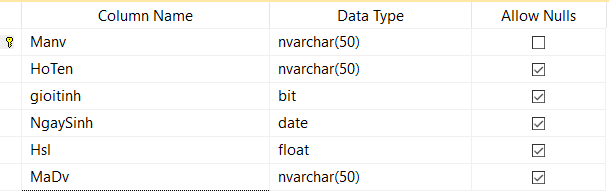
\includegraphics[scale=0.8]{Figures//Hinh34.png}
	\caption{ Cấu trúc của bảng NhanVien }\label{hinh34} 
\end{figure}
\lstset{language=Java,
	tabsize = 4, %% set tab space width
	showstringspaces = false, %% prevent space marking in strings, string is defined as the text that is generally printed directly to the console
	numbers = left, %% display line numbers on the left
	commentstyle = \color{green}, %% set comment color
	keywordstyle = \color{blue}, %% set keyword color
	stringstyle = \color{red}, %% set string color
	rulecolor = \color{black}, %% set frame color to avoid being affected by text color
	basicstyle = \small \ttfamily , %% set listing font and size
	breaklines = true, %% enable line breaking
	numberstyle = \tiny,
}
\begin{lstlisting}[escapechar=`]
import java.sql.Connection;
import java.sql.DriverManager;
import java.sql.PreparedStatement;
import java.sql.ResultSet;
import java.text.SimpleDateFormat;
import java.util.Date;
public class ViDu382 {
public static void main(String[] args) {
Connection   cn=null;
try { 
	//b1, b2
	cn=DungChung.KetNoi();
	//b3: `Đặt chế độ AutoCommi=false`
	cn.setAutoCommit(false);
	//b4: `Tạo bảng NhanVien(MaNv,HoTen,GioiTinh,NgaySinh,HSL,Madv)`
	//`Tạo câu lệnh SQL để tạo bảng NhanVien`
	String sql="CREATE TABLE NhanVien(MaNv nvarchar(15) NOT NULL,HoTen nvarchar(50) NULL,GioiTinh bit NULL,	NgaySinh date NULL,	Hsl real NULL,	MaDv [nvarchar](50) NULL, PRIMARY KEY( MaNv ))";
	PreparedStatement cmd= cn.prepareStatement(sql);
	cmd.executeUpdate();//`Thực thi câu lệnh`
	//b5: `Thêm vào một nhân viên`
	//`Tạo câu lệnh SQL`
	sql="insert into nhanvien(Manv,HoTen,GioiTinh,NgaySinh, Hsl, Madv) values(?,?,?,?,?,?)";
	cmd= cn.prepareStatement(sql);
	//`Thiết lập các tham số`
	cmd.setString(1,"Nv1");
	cmd.setString(2,"`Nguyễn Hoàng Hà`");
	cmd.setBoolean(3,true);
	String ngaysinh ="18/11/1976";
	//`Đổi chuỗi ngaysinh ra kiểu ngày java.util.Date;`
	SimpleDateFormat dd= new SimpleDateFormat("dd/MM/yyyy");
	Date NsUtil=dd.parse(ngaysinh);
	//`Đổi ngày java.util.Date ra java.sql.Date`
	java.sql.Date NsSql= new java.sql.Date(NsUtil.getTime());
	//`Thiết lập tham số cho trường NgaySinh` 
	cmd.setDate(4,NsSql);
	cmd.setDouble(5, 2.34);
	cmd.setString(6, "cntt");
	cmd.executeUpdate();//`Thực thi câu lệnh`
	//b6 `Quyết định thực thi các công việc ở b4,b5`
	cn.commit();//
	cmd.close();//`Giải phóng bộ nhớ`
	cn.close();//`Đóng kết nối`
	System.out.println("`Đã hoàn thành các công việc`");

} catch (Exception e) {
	System.out.print("`Chương trình bị lỗi`");
	try { 
		//b6: `Phục hồi lại công việc ở ở B4`
		cn.rollback();
		cn.close();//`Đóng kết nối`
	} catch (Exception e2) {
		System.out.print("`Không thể phục hồi`");
	}
   }
  }
}
\end{lstlisting}


\section{Đối tượng ResultSet}
Phương thức executeQuery của PrepareStatement hoặc Statement trả về một con trỏ trỏ đến một tập kết quả lấy về từ cơ sở dữ liệu, con trỏ này có kiểu là ResultSet. Người lập trình sử dụng con trỏ này để lấy dữ liệu về, di chuyển con trỏ, cập nhật lại dữ liệu, ...

\subsection{Lấy giá trị của mẫu tin tại vị trí của con trỏ.}
Để lấy giá trị của mẫu tin tại vị trí của con trỏ ta sử dụng các phương thức getXXX. Cú pháp chung của các phương thức này có dạng:
\begin{center}
	 \textbf{public XXX getXXX(int columnIndex)} 
\end{center}
hoặc
\begin{center}
	 \textbf{public XXX getXXX( String columnName)} 
\end{center}

Trong đó, \textbf{XXX} là tên kiểu dữ liệu, \textbf{columnIndex} và \textbf{columnName} là chỉ số của cột hoặc tên cột cần lấy dữ liệu ra. 

Ví dụ: getInt, getString, getDouble, getBoolean, getDate,  ... 

Các phương thức sau lấy ra số nguyên và chuỗi tại vị trí con trỏ:

\textbf{1. public int getInt(int columnIndex):}	được sử dụng để lấy về một số nguyên trên cột thứ columnIndex tại vị trí của con trỏ. Chú ý: cột đầu tiên có số thứ tự là 1.

\textbf{2. public int getInt(String columnName):} được sử dụng để lấy về một số nguyên trên cột có tên columnName tại vị trí của con trỏ.

\textbf{3. public String getString(int columnIndex):}	được sử dụng để lấy về một chuỗi trên cột thứ columnIndex tại vị trí của con trỏ.

\textbf{4. public String getString(String columnName):}	được sử dụng để lấy về một chuỗi trên cột có tên columnName tại vị trí của con trỏ.

\subsection{Các phương thức di chuyển con trỏ mẫu tin}

\textbf{1. public boolean next():}	được sử dụng để di chuyển con trỏ đến mẫu tin tiếp theo từ vị trí hiện tại. Hàm trả về false nếu con trỏ đang đứng mẫu tin cuối cùng mà tiếp tục di chuyển, ngược lại hàm trả về true.

Chú ý: Để duyệt từ mẫu tin đầu tiên đến cuối cùng trong ResultSet: rs ta thường dùng vong lặp while:
\begin{lstlisting}[escapechar=`]
   while (rs.next()){
     //`Xử lý dữ liệu`
   }

\end{lstlisting}

Ví dụ 3.9.1: 
Giả sử bảng NhanVien đã có dữ liệu như Hình \ref{hinh35}
\begin{figure}[!ht]
	\centering
	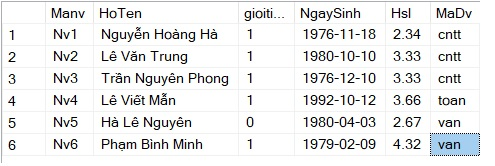
\includegraphics[scale=0.9]{Figures//Hinh35.png}
	\caption{ Dữ liệu của bảng NhanVien }\label{hinh35} 
\end{figure}

Viết chương trình hiển thị thông tin của tất cả các nhân viên trong bảng NhanVien.
\lstset{language=Java,
	tabsize = 4, %% set tab space width
	showstringspaces = false, %% prevent space marking in strings, string is defined as the text that is generally printed directly to the console
	numbers = left, %% display line numbers on the left
	commentstyle = \color{green}, %% set comment color
	keywordstyle = \color{blue}, %% set keyword color
	stringstyle = \color{red}, %% set string color
	rulecolor = \color{black}, %% set frame color to avoid being affected by text color
	basicstyle = \small \ttfamily , %% set listing font and size
	breaklines = true, %% enable line breaking
	numberstyle = \tiny,
}
\begin{lstlisting}[escapechar=`]
import java.sql.*;
import java.text.SimpleDateFormat;
import java.util.Date;
public class ViDu391 {
public static void main(String[] args) {
	Connection   cn=null;
	try { 
		cn=DungChung.KetNoi();
	   	//`Tạo câu lệnh SQL Lấy về tất cả các nhân viên`
		String sql="select * from nhanvien";
		PreparedStatement cmd= cn.prepareStatement(sql);
		ResultSet rs= cmd.executeQuery();//`Thực thi câu lệnh`
		int i=1;
		//`Duyệt qua từng mẫu tin trong rs`
		while(rs.next()){
			String Manv=rs.getString("Manv");//`Lấy ra MaNv`
			String Hoten=rs.getString("HoTen");//`Lấy ra HoTen`
			Boolean GioiTinh=rs.getBoolean("GioiTinh");
			Date NgaySinh =rs.getDate("NgaySinh");
			String Madv=rs.getString("MaDv");
			System.out.println("`Thông tin của nhân viên thứ:`  "+ i++);
			System.out.print(Manv);
			System.out.print(" "+ Hoten);
			System.out.print(" "+ GioiTinh);
			System.out.print(" "+ NgaySinh);
			System.out.println(" "+Madv);
			System.out.println("-------------------");
		}
		rs.close();//` Đóng ResultSet `
		cn.close();//`Đóng kết nối`
		System.out.println("`Đã hoàn thành các công việc`");
	
	} catch (Exception e) {
		System.out.print("`Chương trình bị lỗi`");
		try { 
			cn.close();//`Đóng kết nối`
		} catch (Exception e2) {
			System.out.print("`Không thể phục hồi`");
		}
    }
  }
}
\end{lstlisting}

Kết quả hiển thị của chương trình:

\begin{figure}[!ht]
	\centering
	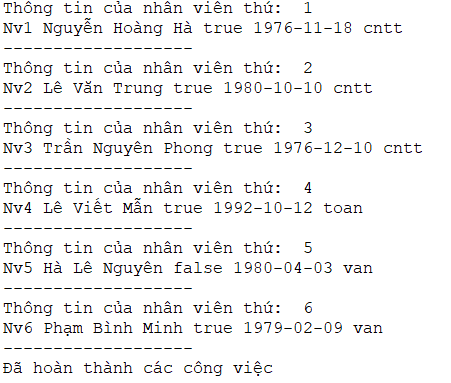
\includegraphics[scale=0.9]{Figures//Hinh36.png}
	\caption{ Kết quả chương trình }\label{hinh36} 
\end{figure}

 
\textbf{2. public boolean previous():}	được sử dụng để di chuyển con trỏ đến một mẫu tin trước đó từ vị trí hiện tại.

\textbf{3. public boolean first():}	được sử dụng để di chuyển con trỏ đến mẫu tin đầu tiên.

\textbf{4. public boolean last():}	được sử dụng để di chuyển con trỏ đến mẫu tin cuối cùng.

\textbf{5. public boolean absolute(int row):}	được sử dụng để di chuyển con trỏ đến số mẫu tin thứ row.

\textbf{6. public boolean relative(int row):}	được sử dụng để di chuyển con trỏ đến mẫu tin tương đối. Nếu row là số âm thì di chuyển con trỏ đến mẫu tin trước mẫu tin hiện tại, ngược lại di chuyển mẫu tin đến sau mẫu tin hiện tại.

\textbf{7. public void moveToInsertRow() }

Di chuyển con trỏ tới một hàng đặc biệt trong ResultSet mà có thể được sử dụng để chèn một hàng mới vào trong cơ sở dữ liệu. 

Chú ý: Để di chuyển con trỏ mẫu tin bằng các phương thức previous(), first(), last(), absolute(), relative(), moveToInsertRow() ta phải chỉ rõ loại ResultSet (resultsetType) và kiểu của ResultSet (resultSetConcurrency) trong phương thức prepareStatement:

\textbf{public PreparedStatement prepareStatement(String sql, int resultSetType, int resultSetConcurrency)throws SQLException}

Trong đó: 
resultsetType: chỉ dùng  1 trong 2 kiểu:
\begin{itemize}
	\item ResultSet.TYPE \text{\_}SCROLL \text{\_}INSENSITIVE
	\item ResultSet.TYPE \text{\_}SCROLL \text{\_}SENSITIVE
\end{itemize}
resultSetConcurrency là 1 trong 2 kiểu:
\begin{itemize}
	\item ResultSet.CONCUR \text{\_}READ \text{\_}ONLY:
	\item ResultSet.CONCUR \text{\_}UPDATABLE: 
\end{itemize}

Ví dụ 3.9.2. Giả sử bảng NhanVien đã có dữ liệu như Hình \ref{hinh35}. Hãy hiển thị họ tên của người đầu tiên, người cuối cùng, người thứ 4, người đứng trước 2 mẫu tin tính từ mẫu tin số 4. người đứng sau 2 mẫu tin tính từ mẫu tin số 4.

\lstset{language=Java,
	tabsize = 4, %% set tab space width
	showstringspaces = false, %% prevent space marking in strings, string is defined as the text that is generally printed directly to the console
	numbers = left, %% display line numbers on the left
	commentstyle = \color{green}, %% set comment color
	keywordstyle = \color{blue}, %% set keyword color
	stringstyle = \color{red}, %% set string color
	rulecolor = \color{black}, %% set frame color to avoid being affected by text color
	basicstyle = \small \ttfamily , %% set listing font and size
	breaklines = true, %% enable line breaking
	numberstyle = \tiny,
}
\begin{lstlisting}[escapechar=`]
import java.sql.Connection;
import java.sql.DriverManager;
import java.sql.PreparedStatement;
import java.sql.ResultSet;

import dao.DungChung;
public class ViDu392 {
public static void main(String[] args) {
	Connection   cn=null;
	try { 
		cn=DungChung.KetNoi();
		//`Tạo câu lệnh SQL Lấy về tất cả các nhân viên`
		String sql="select * from nhanvien";
		PreparedStatement cmd= cn.prepareStatement(sql, ResultSet .TYPE_SCROLL_INSENSITIVE, ResultSet.CONCUR_READ_ONLY);
		//`Thực thi câu lệnh`
		ResultSet rs= cmd.executeQuery();
		//`Đưa con trỏ về mẫu tin đầu tiên;`
		rs.first();
		//`Lấy ra HoTen mẫu tin thứ 1`
		String Hoten=rs.getString("HoTen");
		System.out.println("`Họ tên người đầu tiên:` "+ Hoten);
		System.out.println("-------------------");
		
		//`Đưa con trỏ về mẫu tin cuối cùng;`
		rs.last();
		//`Lấy ra HoTen mẫu tin thứ cuối cùng`
		Hoten=rs.getString("HoTen");
		System.out.println("`Họ tên người cuối cùng:` "+ Hoten);
		System.out.println("-------------------");
		//`Đưa con trỏ về mẫu tin thứ 4`;
		rs.absolute(4);
		//`Lấy ra HoTen mẫu tin thứ 4`
		Hoten=rs.getString("HoTen");
		System.out.println("`Họ tên người người thứ 4:` "+ Hoten);
		System.out.println("-------------------");
		
		//`Đưa con trỏ về trước 2 mẫu tin tính từ mẫu tin số 4`
		rs.absolute(4);
		rs.relative(-2);
		//`Lấy ra HoTen mẫu tin thứ 2`
		Hoten=rs.getString("HoTen");
		System.out.println("`Họ tên người thứ 2:` "+ Hoten);
		System.out.println("-------------------");
		
		//`Đưa con trỏ về sau 2 mẫu tin tính từ mẫu tin số 4`
		rs.absolute(4);
		rs.relative(2);
		//`Lấy ra HoTen mẫu tin thứ 6`
		Hoten=rs.getString("HoTen");
		System.out.println("`Họ tên người thứ 6: `"+ Hoten);
		System.out.println("-------------------");
		rs.close();//` Đóng ResultSet `
		cn.close();//`Đóng kết nối`
		System.out.println("`Đã hoàn thành các công việc`");
	
	} catch (Exception e) {
		e.printStackTrace();
		System.out.print("`Chương trình bị lỗi`");
	}
 }
}

\end{lstlisting}
Kết quả hiển thị của chương trình:

\begin{figure}[!ht]
	\centering
	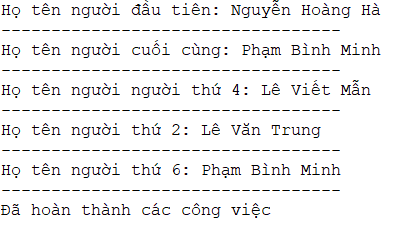
\includegraphics[scale=0.9]{Figures//Hinh37.png}
	\caption{ Kết quả chương trình }\label{hinh37} 
\end{figure}

\subsection{Các phương thức cập nhật dữ liệu}

Để cập nhật dữ liệu trong ResultSet, ta sử dụng phương thức có dạng:
\begin{center}
	\textbf{ public void updateXXX(int columnIndex, XXX value);}
\end{center}	
	hoặc
\begin{center}	
	\textbf{ public void updateXXX( String columnName, XXX value);} 
\end{center}
Trong đó, \textbf{XXX} là tên kiểu dữ liệu; \textbf{columnIndex} và \textbf{columnName} là chỉ số của cột hoặc tên cột cần cập nhật dữ liệu; value là giá trị cần cập nhật. ví dụ: updateInt, updateString, updateDouble, updateDate, ...

Để cập nhật dữ liệu vào CSDL, khi lấy dữ liệu về ta phải sử dụng kiểu con trỏ (resultSetType) là ResultSet.TYPE\_SCROLL\_ SENSITIVE và loại con trỏ (resultSetConcurrency) là ResultSet.CONCUR\_ UPDATABLE.

Các phương thức update này không cập nhật vào cơ sở dữ liệu. Để cập nhật dữ liệu vào cơ sở dữ liệu, ta sử dụng thêm phương thức updateRow() hoặc insertRow() nếu thêm mới 1 mẫu tin.

\textbf{Một số phương thức thường dùng để cập nhật dữ liệu:}

\textbf{1. public void updateInt(int columnIndex hoặc String \\ columnName, int x):}

Cập nhật giá trị nguyên \textbf{x} vào mẫu tin hiện tại của cột có chỉ số \textbf{columnIndex} hoặc có tên cột là \textbf{columnName}.

\textbf{2. public void updateString(int columnIndex hoặc String columnName, String x)}

Cập nhật chuỗi \textbf{x} vào mẫu tin hiện tại của cột có chỉ số \textbf{columnIndex} hoặc có tên cột là \textbf{columnName}.

\textbf{3. public void updateBoolean(int columnIndex hoặc String columnName, Boolean x)}

Cập nhật giá trị \textbf{x} vào mẫu tin hiện tại của cột có chỉ số \textbf{columnIndex} hoặc có tên cột là \textbf{columnName}

\textbf{4. public void updateDate(int columnIndex hoặc String columnName, Date x)}

Cập nhật ngày \textbf{x} vào mẫu tin hiện tại của cột có chỉ số \textbf{columnIndex} hoặc có tên cột là \textbf{columnName}

\textbf{5. public void updateDouble(int columnIndex hoặc String columnName, Double x)}

Cập nhật số thực \textbf{x} vào mẫu tin hiện tại của cột có chỉ số \textbf{columnIndex} hoặc có tên cột là \textbf{columnName}

Ví dụ 3.9.3. Viết chương trình để nhập vào 1 mã nhân viên. Tìm xem có nhân viên có mã này hay không. Nếu có thì nhập vào 1 ngày sinh và cập nhập lại ngày sinh cho nhân viên tìm được.
\lstset{language=Java,
	tabsize = 4, %% set tab space width
	showstringspaces = false, %% prevent space marking in strings, string is defined as the text that is generally printed directly to the console
	numbers = left, %% display line numbers on the left
	commentstyle = \color{green}, %% set comment color
	keywordstyle = \color{blue}, %% set keyword color
	stringstyle = \color{red}, %% set string color
	rulecolor = \color{black}, %% set frame color to avoid being affected by text color
	basicstyle = \small \ttfamily , %% set listing font and size
	breaklines = true, %% enable line breaking
	numberstyle = \tiny,}
\begin{lstlisting}[escapechar=`]
import java.sql.Connection;
import java.sql.PreparedStatement;
import java.sql.ResultSet;
import java.text.SimpleDateFormat;
import java.util.Date;
import java.util.Scanner;

import dao.DungChung;
public class ViDu3_9_3 {

public static void main(String[] args) {
Connection   cn=null;
try { 
	//`Kết nối vào CSDL`
	cn=DungChung.KetNoi();
	//`Nhập vào từ bàn phím 1 mã nhân viên`
	System.out.println("`Nhập vào 1 mã nhân viên:`");
	Scanner nhap= new Scanner(System.in);
	String manv=nhap.next();
	
	//`Tạo câu lệnh SQL để lấy về nhân viên có mã là manv`
	String sql="select * from nhanvien where Manv=?";
	//`Tạo câu lệnh prepareStatement với:`
	//`Kiểu con trỏ: TYPE\_SCROLL\_SENSITIVE`
	// `và loại con trỏ: CONCUR\_UPDATABLE`
	PreparedStatement cmd= cn.prepareStatement(sql,ResultSet.TYPE_SCROLL_SENSITIVE, ResultSet.CONCUR_UPDATABLE);
	//`Truyền tham số vào câu lệnh`
	cmd.setString(1, manv);
	//`Thực thi câu lệnh`
	ResultSet rs= cmd.executeQuery();
	
	//`Nếu trong rs không có dữ liệu`
	if (!rs.next())
		System.out.println("`Không tim ra nhân viên này`");
	else{
		System.out.println("`Nhập vào 1 ngày sinh theo dạng: yyyy-MM-dd`");
		String ngay=nhap.next();
		//`Đổi chuỗi sang ngày của Util`
		SimpleDateFormat dd= new SimpleDateFormat( "yyyy-MM-dd");
		Date ngayUtil=dd.parse(ngay);
		//`Đổi ngày của Util sang ngày của sql `
		//`và cập nhật lại ngày sinh`
		rs.updateDate("NgaySinh", new java.sql.Date( ngayUtil.getTime()));
		rs.updateRow();
	}
	rs.close();//` Đóng ResultSet `
	cn.close();//`Đóng kết nối`
} catch (Exception e) {
	e.printStackTrace();
	System.out.print("`Chương trình bị lỗi`");
   }
  }
}
\end{lstlisting}
\subsection{Thêm và xóa một mẫu tin}
Để thêm một mẫu tin vào cơ sở dữ liệu thì ta thực hiện các bước:
\begin{itemize}
	\item Di chuyển con trỏ về sau mẫu tin cuối cùng và tạo ra 1 mẫu tin: moveToInsertRow();
	\item Cập nhật lại dữ liệu vào mẫu tin mới thêm, sử dụng các phương thức updateXXX(int columnIndex, XXX value);
	\item Lưu dữ liệu vào cơ sở dữ liệu, sử dụng phương thức insertRow();
\end{itemize}
Ví dụ 3.9.4. Viết chương trình để thêm vào 1 nhân viên.
\lstset{language=Java,
	tabsize = 4, %% set tab space width
	showstringspaces = false, %% prevent space marking in strings, string is defined as the text that is generally printed directly to the console
	numbers = left, %% display line numbers on the left
	commentstyle = \color{green}, %% set comment color
	keywordstyle = \color{blue}, %% set keyword color
	stringstyle = \color{red}, %% set string color
	rulecolor = \color{black}, %% set frame color to avoid being affected by text color
	basicstyle = \small \ttfamily , %% set listing font and size
	breaklines = true, %% enable line breaking
	numberstyle = \tiny,}
\begin{lstlisting}[escapechar=`]
import java.sql.*;
import java.text.SimpleDateFormat;
import java.util.Date;
import java.util.Scanner;

import dao.DungChung;
public class ViDu3_9_4 {

public static void main(String[] args) {
Connection   cn=null;
try { 
	//`Kết nối vào CSDL`
	cn=DungChung.KetNoi();
	//`Nhập vào từ bàn phím 1 mã nhân viên`
	System.out.println("`Nhập vào 1 mã nhân viên:`");
	Scanner nhap= new Scanner(System.in);
	String manv=nhap.nextLine();
	//`Tạo câu lệnh SQL để lấy về nhân viên có mã là manv`
	String sql="select * from nhanvien where Manv=?";
	//`Tạo câu lệnh prepareStatement `
	PreparedStatement cmd= cn.prepareStatement(sql,ResultSet.TYPE_SCROLL_SENSITIVE, ResultSet.CONCUR_UPDATABLE);
	//`Truyền tham số vào câu lệnh`
	cmd.setString(1, manv);
	//`Thực thi câu lệnh`
	ResultSet rs= cmd.executeQuery();
	//`Nếu có dữ liệu trong rs`
	if (rs.next())
		System.out.println("`Đã tồn tại nhân viên có mã: `"+manv);
	else{
		System.out.println("`Nhập  họ tên nhân viên:`");
		String HoTen=nhap.nextLine();
		
		System.out.println("`Nhập giới tính (true/false):`");
		Boolean GioiTinh=Boolean.parseBoolean(nhap.nextLine());
		System.out.println("`Nhập vào 1 ngày sinh theo dạng: yyyy-MM-dd`");
		String ngay=nhap.nextLine();
		//`Đổi chuỗi sang ngày của Util`
		SimpleDateFormat dd= new SimpleDateFormat("yyyy-MM-dd");
		Date ngayUtil=dd.parse(ngay);
		
		System.out.println("`Nhập hệ số lương:`");
		Double hsl= Double.parseDouble(nhap.nextLine());
		
		System.out.println("`Nhập mã đơn vị:`");
		String Madv=nhap.nextLine();
		`//Di chuyển con trỏ về sau mẫu tin cuối cùng và tạo ra 1 mẫu tin`	
		rs.moveToInsertRow();
  		//`Cập nhật lại dữ liệu vào mẫu tin mới thêm`
		rs.updateString("Manv", manv);
		rs.updateString("HoTen", HoTen);
		rs.updateBoolean("GioiTinh", GioiTinh);
		rs.updateDate("NgaySinh", new java.sql.Date(ngayUtil.getTime()));
		rs.updateDouble("Hsl", hsl);
		rs.updateString("MaDv", Madv);
		//`Lưu vào CSDL`
		rs.insertRow();
	}
	
	rs.close();//` Đóng ResultSet `
	cn.close();//`Đóng kết nối`
} catch (Exception e) {
	e.printStackTrace();
	System.out.print("`Chương trình bị lỗi`");
   }
  }
}

\end{lstlisting}


Để xóa một mẫu tin ra khỏi cơ sở dữ liệu thì ta thực hiện các bước:
\begin{itemize}
	\item Di chuyển con trỏ đến mẫu tin cần xóa (tìm mẫu tin cần xóa)
	\item Xóa và lưu dữ liệu vào cơ sở dữ liệu, sử dụng phương thức deleteRow().
\end{itemize}


Ví dụ 3.9.5. Viết chương trình để nhập vào 1 mã nhân viên và xóa nhân viên có mã này ra khỏi CSDL.
\lstset{language=Java,
	tabsize = 4, %% set tab space width
	showstringspaces = false, %% prevent space marking in strings, string is defined as the text that is generally printed directly to the console
	numbers = left, %% display line numbers on the left
	commentstyle = \color{green}, %% set comment color
	keywordstyle = \color{blue}, %% set keyword color
	stringstyle = \color{red}, %% set string color
	rulecolor = \color{black}, %% set frame color to avoid being affected by text color
	basicstyle = \small \ttfamily , %% set listing font and size
	breaklines = true, %% enable line breaking
	numberstyle = \tiny,}
\begin{lstlisting}[escapechar=`]
import java.sql.Connection;
import java.sql.PreparedStatement;
import java.sql.ResultSet;
import java.util.Scanner;
import dao.DungChung;
public class ViDu3_9_5 {
public static void main(String[] args) {
Connection   cn=null;
try { 
		cn=DungChung.KetNoi();//`Kết nối vào CSDL`
	//`Nhập vào từ bàn phím 1 mã nhân viên`
	System.out.println("`Nhập vào 1 mã nhân viên:`");
	Scanner nhap= new Scanner(System.in);
	String manv=nhap.nextLine();
	//`Tạo câu lệnh SQL để lấy về nhân viên có mã là manv`
	String sql="select * from nhanvien where Manv=?";
	//`Tạo câu lệnh prepareStatement `
	PreparedStatement cmd= cn.prepareStatement(sql,ResultSet.TYPE_SCROLL_SENSITIVE, ResultSet.CONCUR_UPDATABLE);
	cmd.setString(1, manv);//`Truyền tham số vào câu lệnh`
	//`Thực thi câu lệnh`
	ResultSet rs= cmd.executeQuery();
	//`Nếu không tim thấy`
	if (!rs.next())
		System.out.println("`Không tìm ra nhân viên có mã:` "+manv);
	else{
		//` Xóa dòng hiện tại và lưu vào CSDL`
		rs.deleteRow();
	}
	rs.close();//` Đóng ResultSet `
	cn.close();//`Đóng kết nối`
} catch (Exception e) {
	e.printStackTrace();
	System.out.print("`Chương trình bị lỗi`");
	}
  }
}

\end{lstlisting}
\subsection{Lấy về bảng mô tả trong ResultSet}
Các phần trên tập trung vào truy xuất dữ liệu trong ResultSet, để lấy thông tin (metadata) trong ResultSet như tên bảng, tổng số cột, tên cột, kiểu của cột, ...ResultSet hỗ trợ hàm:
\textbf{\begin{center}
		public ResultSetMetaData getMetaData();
\end{center}}
 
\textbf{Một số phương thức trong ResultSetMetaData:}

\textbf{1. public int getColumnCount()throws SQLException}:
trả về tổng số cột trong đối tượng ResultSet.

\textbf{2. public String getColumnName(int index)throws SQLException}: trả về tên cột tại chỉ mục đã cho.

\textbf{3. public String getColumnTypeName(int index)throws SQLException
}: trả về tên kiểu của cột tại chỉ mục đã cho.

\textbf{4. public Boolean isAutoIncrement(int column)}

Xác định xem cột đã cho có phải là tự động tăng (auto-increment) hay không.

Ví dụ 3.9.6. Viết hàm GetBang(String TenBang) để hiển thị tên cột và dữ liêu của bảng: TenBang. Sau đó viết chương trình gọi lại hàm GetBang để hiển thi tên cột vào dữ liệu của bảng NhanVien và DonVi.
\lstset{language=Java,
	tabsize = 4, %% set tab space width
	showstringspaces = false, %% prevent space marking in strings, string is defined as the text that is generally printed directly to the console
	numbers = left, %% display line numbers on the left
	commentstyle = \color{green}, %% set comment color
	keywordstyle = \color{blue}, %% set keyword color
	stringstyle = \color{red}, %% set string color
	rulecolor = \color{black}, %% set frame color to avoid being affected by text color
	basicstyle = \small \ttfamily , %% set listing font and size
	breaklines = true, %% enable line breaking
	numberstyle = \tiny,}
\begin{lstlisting}[escapechar=`]
import java.sql.PreparedStatement;
import java.sql.ResultSet;
import java.sql.ResultSetMetaData;

public class ViDu3_9_6 {
public static  void GetBang(String TenBang) throws Exception{
	Connection cn=DungChung.KetNoi();//`Tạo đường kết nối`
	//` Tạo câu lênh SQl để lấy về dữ liệu của bảng: TenBang`
	String sql="select * from "+ TenBang;
	//`Tạo và thực thi câu lệnh`
	PreparedStatement cmd=cn.prepareStatement(sql);
	ResultSet rs=cmd.executeQuery();
	//` Lấy về thông tin của rs (metadata)`
	ResultSetMetaData meta=rs.getMetaData();
	//'` Lấy về tổng số cột`
	int sc=meta.getColumnCount();
	//` Hiển thị tên các cột của bảng: TenBang`
	for(int i=1;i<=sc;i++)
		System.out.printf("%-20s",meta.getColumnName(i));
	System.out.println();
	// `Duyệt qua các mẫu tin trong rs`
	while(rs.next()){
		//` Duyệt qua các cột trên mỗi mẫu tin`
		for(int i=1;i<=sc;i++)
			//` Hiển thị giá trị trên cột i`
			System.out.printf("%-20s",rs.getString(i));
		System.out.println();
	}
	rs.close();
	cn.close();
}
public static void main(String[] args) {
try {
	System.out.println("`Bảng Nhân viên:`");
	DungChung.GetBang("NhanVien");
	System.out.println("`Bản Đơn Vị:`");
	DungChung.GetBang("DonVi");
} catch (Exception e) {
	e.printStackTrace();
  }
 }
}
\end{lstlisting}
Kết quả hiển thị của chương trình như Hình \ref{hinh38}

	\begin{figure}[!ht]
	\centering
	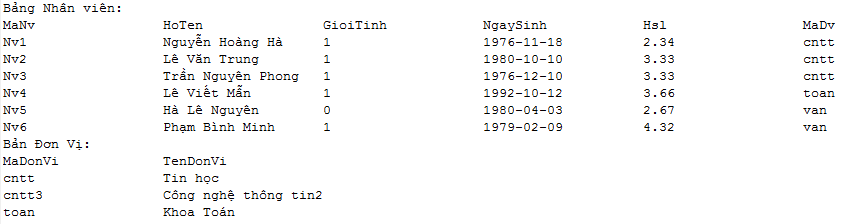
\includegraphics[scale=0.5]{Figures//Hinh38.png}
	\caption{ Dữ liệu bảng Nhân viên và Đơn vị }\label{hinh38} 
\end{figure}
\section{Bài tập thực hành}
Để quản lý nhân viên của một công ty người ta quản lý đơn vị và nhân viên của các đơn vị. Đối với đơn vị cần quản lý mã đơn vị và tên đơn vị, đối với nhân viên người ta quản lý các thông tin: mã nhân viên, họ tên, ngày sinh, giới tính, hệ số lương (hsl), mã đơn vị và mật khẩu. \\
\textbf{Yêu cầu của bài toán}:\\
Đối với đơn vị cần có các chức năng:
\begin{enumerate}
	\item Hiển thị tất cả các đơn vị.
	\item Thêm, xóa và sửa các đơn vị.
	\item Tìm kiếm theo tên đơn vị.
\end{enumerate}
Đối với nhân viên cần có các chức năng:
\begin{enumerate}
	\item Thêm, xóa và đổi mật khẩu các nhân viên.
	\item Hiển thị các nhân viên theo đơn vị.
	\item Tìm kiếm nhân viên theo mã đơn vị hoặc họ tên.
	\item Tìm kiếm nhân viên theo mã nhân viên.
	\item Cho nhân viên đăng nhập vào hệ thống.
\end{enumerate}

Để thực hiện các chức năng của bài toán, sinh viên làm các bài thực hành sau:
\subsection{Bài thực hành 1}
 - Hãy thiết lập cấu hình để SQL Server cho phép đăng nhập bằng tài khoản sa với mật khẩu bất kỳ.
 
 - Hãy mở giao thức TCP/IP và cổng 1433 cho SQL Server.
 
 - Tạo cơ sở dữ liệu: Qlnv bao gồm 2 bảng donvi và nhanvien có quan hệ như   Hình \ref{hinh39_1}:
 
 \begin{figure}[!ht]
 	\centering
 	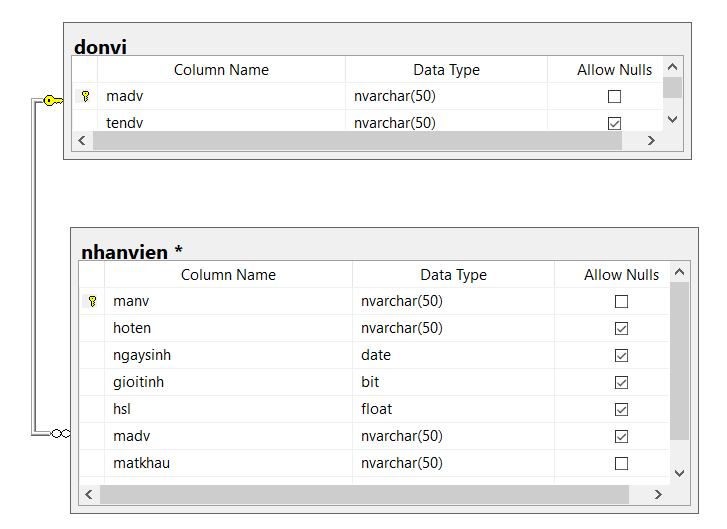
\includegraphics[scale=0.7]{Figures//Hinh39_1.png}
 	\caption{ Lược đồ quan hệ giữa các bảng }\label{hinh39_1} 
 \end{figure}
 
 - Hãy nhập dữ liệu vào bảng donvi và nhanvien.
\subsection{Bài thực hành 2}
\textbf{1. Tạo các gói}

Sử dụng Eclipse để tạo các Source Folder và các gói như Hình \ref{hinh39}.
	\begin{figure}[!ht]
	\centering
	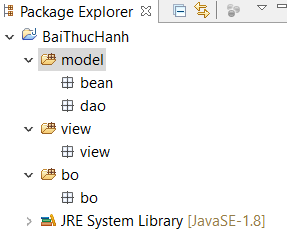
\includegraphics[scale=0.9]{Figures//Hinh39.png}
	\caption{ Các gói trong Project }\label{hinh39} 
\end{figure}

\textbf{Nhiệm vụ của mỗi gói:}

\textbf{model:} Chứa các gói và lớp tách riêng với tầng bo (business objects) và tầng view:

\textbf{model.bean: } Chứa các thực thể, gồm các trường (private), kèm theo các phương thức set/get, hàm tạo, ...

\textbf{model.dao:} Thực hiện các công việc liên quan đến CSDL như kết nối, lấy dữ liệu, truy vấn, chỉnh sửa, thêm xóa dữ liệu trực tiếp với cơ sở dữ liệu

\textbf{bo: }
Truyền yêu cầu từ view chuyển qua dao, lấy dữ liệu từ dao về cho view. Nhiệm vụ của tầng này là xử lý các yêu cầu nghiệp vụ.

\textbf{view:} Dùng để nhập xuất dữ liệu của người dùng.

Một số quy tắc tương tác giữa các gói như thể hiện ở Hình \ref{hinh319}:
	\begin{figure}[!ht]
	\centering
	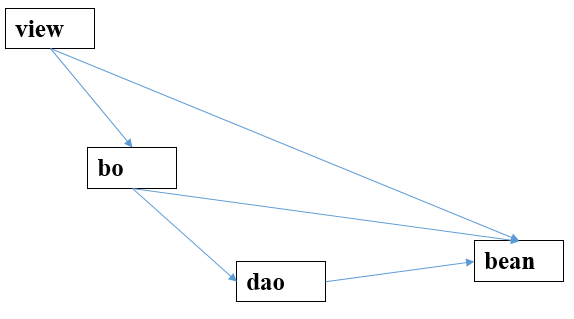
\includegraphics[scale=0.9]{Figures//Hinh319.png}
	\caption{ Quan hệ giữa các gói }\label{hinh319} 
\end{figure}

Trong đó:

\textbf{bean} chứa các thực thể, có thể sử dụng ở bất cứ nơi nào cần thiết như: \textbf{dao}, \textbf{bo} và \textbf{view}.

Các kết nối đến CSDL chỉ thực hiện ở \textbf{model.dao}, các tầng khác không liên quan đến CSDL.

\textbf{dao} chỉ cho phép gọi từ \textbf{bo}, các nơi khác không được gọi đến \textbf{dao}.

\textbf{bo} chỉ cho phép gọi từ \textbf{view}, các nơi khác không được gọi \textbf{bo}.

\textbf{view}: chỉ nhận và gửi dữ liệu từ \textbf{bo}.\\
\textbf{2. Lập trình trên gói bean}

Tại \textbf{model.bean}, hãy tạo ra lớp sau:

a. Lớp \textbf{donvibean} bao gồm các trường và phương thức như sau:

\lstset{language=Java,
	tabsize = 4, %% set tab space width
	showstringspaces = false, %% prevent space marking in strings, string is defined as the text that is generally printed directly to the console
	numbers = left, %% display line numbers on the left
	commentstyle = \color{green}, %% set comment color
	keywordstyle = \color{blue}, %% set keyword color
	stringstyle = \color{red}, %% set string color
	rulecolor = \color{black}, %% set frame color to avoid being affected by text color
	basicstyle = \small \ttfamily , %% set listing font and size
	breaklines = true, %% enable line breaking
	numberstyle = \tiny,}
\begin{lstlisting}[escapechar=`]
package bean;
public class donvibean {
	//` Khai báo 2 trường madv và tendv`
	private String madv;
	private String tendv;
	//` Tạo constructor không tham số`
	public donvibean() {
		super();
	}
	//`Tạo constructor có đầy đủ tham số`
	public donvibean(String madv, String tendv) {
		super();
		this.madv = madv;
		this.tendv = tendv;
	}
	//`lần lượt viết các hàm để lấy giá tri ra (get)`
	//`và gán giá trị vào (set) các trường`
	public String getMadv() {
		return madv;
	}
	public void setMadv(String madv) {
		this.madv = madv;
	}
	public String getTendv() {
		return tendv;
	}
	public void setTendv(String tendv) {
		this.tendv = tendv;
	}
	//`Viết hàm tostring() để hiển thị giá trị các trường`
	@Override
	public String toString() {
		return madv + " " + tendv ;
}
}
\end{lstlisting}

Để kiểm tra các trường và phương thức trên lớp \textbf{donvibean}, mở lớp \textbf{donvibean} và thêm vào hàm \textbf{main()} để tạo ra 1 đơn vị và hiển thị thông tin của đơn vị vừa tạo:

\lstset{language=Java,
	tabsize = 4, %% set tab space width
	showstringspaces = false, %% prevent space marking in strings, string is defined as the text that is generally printed directly to the console
	numbers = left, %% display line numbers on the left
	commentstyle = \color{green}, %% set comment color
	keywordstyle = \color{blue}, %% set keyword color
	stringstyle = \color{red}, %% set string color
	rulecolor = \color{black}, %% set frame color to avoid being affected by text color
	basicstyle = \small \ttfamily , %% set listing font and size
	breaklines = true, %% enable line breaking
	numberstyle = \tiny,}
\begin{lstlisting}[escapechar=`]
 public static void main(String[] args) {
 	//` tạo ra một đơn vị`
 	 donvibean dv= new donvibean("cntt","`Công nghệ thông tin`");
 	 //` hiển thị thông tin của đơn vị`
	 System.out.println(dv.toString());
 }
\end{lstlisting}

\textbf{Chú ý:}
Trên Eclipse có sẵn chức năng phát sinh ra mã lệnh, đối với mỗi lớp trên \textbf{model.bean} chúng ta chỉ cần gõ tên trường, sau đó Eclipse sẽ tự động sinh ra hàm tạo, hàm toString(), các hàm get/set tương ứng với từng trường. 

Ví dụ: trong lớp \textbf{donvibean} sau khi gõ 2 trường madv và tendv, chúng ta phát sinh ra hàm tạo, hàm get/set, hàm toString() như sau:

Chọn vị trí cần phát sinh ra mã lệnh, kích chuột phải và chọn Source, sau đó chọn các chức năng phát sinh tương ứng như Hình \ref{hinh320}, trong đó:

(1): phát sinh các hàm get/set;

(2): phát sinh hàm toString();

(3): phát sinh hàm tạo với các tham số;

(4): phát sinh hàm tạo không tham số.

\begin{figure}[!ht]
	\centering
	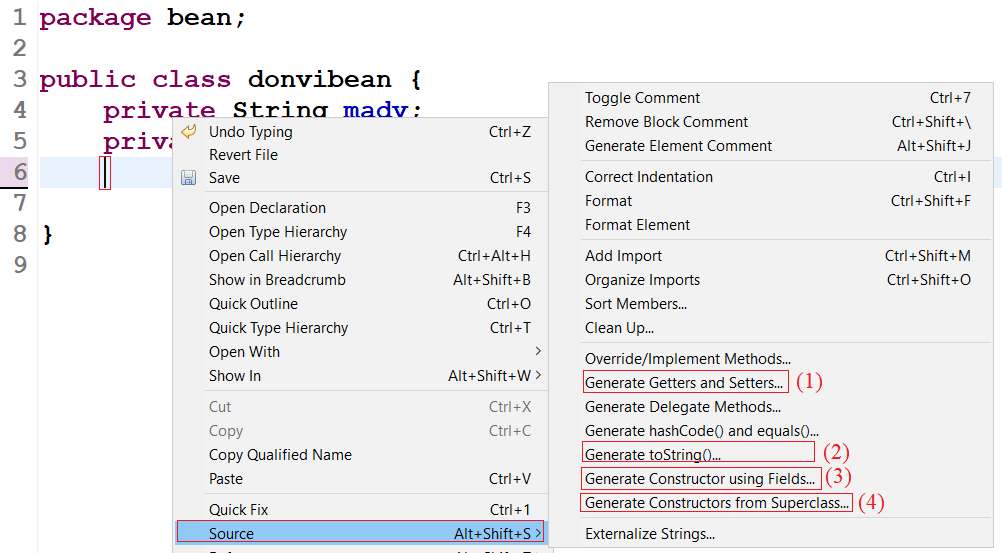
\includegraphics[scale=0.6]{Figures//Hinh320.png}
	\caption{ Phát sinh các hàm trên Eclipse }\label{hinh320} 
\end{figure}

b. Lớp \textbf{nhanvienbean}

Tương tự như lớp \textbf{donvibean}, hãy tạo lớp \textbf{nhanvienbean} bao gồm các trường và phát sinh các phương thức như sau:

\lstset{language=Java,
	tabsize = 4, %% set tab space width
	showstringspaces = false, %% prevent space marking in strings, string is defined as the text that is generally printed directly to the console
	numbers = left, %% display line numbers on the left
	commentstyle = \color{green}, %% set comment color
	keywordstyle = \color{blue}, %% set keyword color
	stringstyle = \color{red}, %% set string color
	rulecolor = \color{black}, %% set frame color to avoid being affected by text color
	basicstyle = \small \ttfamily , %% set listing font and size
	breaklines = true, %% enable line breaking
	numberstyle = \tiny,}
\begin{lstlisting}[escapechar=`]
package bean;
import java.util.Date;
public class nhanvienbean {
	private String manv;
	private String hoten;
	private Date ngaysinh;
	private Boolean gioitinh;
	private Double hsl;
	private String madv;
	private String matkhau;
	public nhanvienbean() {
		super();
	}
	public nhanvienbean(String manv, String hoten, Date ngaysinh, Boolean gioitinh,Double hsl, String madv, String matkhau) {
		super();
		this.manv = manv;
		this.hoten = hoten;
		this.ngaysinh = ngaysinh;
		this.gioitinh = gioitinh;
		this.hsl = hsl;
		this.madv = madv;
		this.matkhau = matkhau;
	}
	public String getManv() {
		return manv;
	}
	public void setManv(String manv) {
		this.manv = manv;
	}
	public String getHoten() {
		return hoten;
	}
	public void setHoten(String hoten) {
		this.hoten = hoten;
	}
	public Date getNgaysinh() {
		return ngaysinh;
	}
	public void setNgaysinh(Date ngaysinh) {
		this.ngaysinh = ngaysinh;
	}
	public Boolean getGioitinh() {
		return gioitinh;
	}
	public void setGioitinh(Boolean gioitinh) {
		this.gioitinh = gioitinh;
	}
	public Double getHsl() {
		return hsl;
	}
	public void setHsl(Double hsl) {
		this.hsl = hsl;
	}
	public String getMadv() {
		return madv;
	}
	public void setMadv(String madv) {
		this.madv = madv;
	}
	public String getMatkhau() {
		return matkhau;
	}
	public void setMatkhau(String matkhau) {
		this.matkhau = matkhau;
}
}
\end{lstlisting}

\textbf{Yêu cầu bổ sung:}

Để kiểm tra các trường và phương thức trên lớp \textbf{nhanvienbean}, mở lớp \textbf{nhanvienbean} và sinh viên hãy thêm vào hàm \textbf{main()} để tạo ra 1 nhân viên bất kỳ và hiển thị thông tin của nhân viên vừa tạo.\\
\textbf{3. Lập trình trên gói dao}

Tại \textbf{model.dao}, hãy tạo ra lớp để thực hiện các công việc liên quan đến CSDL như kết nối, lấy dữ liệu, truy vấn, chỉnh sửa, thêm xóa dữ liệu trực tiếp với cơ sở dữ liệu. Trong gói \textbf{dao} này sẽ tạo ra các lớp sau:
\begin{itemize}
	\item Lớp \textbf{DungChung}: gồm các phương thức dùng chung trong gói \textbf{dao}  như kết nối vào cơ sở dữ liệu, lấy về tên cột của một bảng, lấy về dữ liệu của một bảng.
	\item Lớp \textbf{donvidao}: gồm các phương thức thao tác trên bảng \textbf{donvi} như lấy về tất cả các đơn vị, thêm, xóa, ...
	\item Lớp \textbf{nhanviendao}: gồm các phương thức thao tác trên bảng \textbf{nhanvien} như lấy về tất cả các nhân viên, thêm, ...
\end{itemize}
\textbf{ a. Xây dựng lớp DungChung}
 
 Lớp này bao gồm các phương thức:
\begin{itemize}
	\item Kết nối vào cơ sỡ dữ liệu;
	\item Lấy dữ liệu của một bảng bất kỳ;
	\item Lấy về các tên cột của một bảng bất kỳ.
\end{itemize}

  
\lstset{language=Java,
	tabsize = 4, %% set tab space width
	showstringspaces = false, %% prevent space marking in strings, string is defined as the text that is generally printed directly to the console
	numbers = left, %% display line numbers on the left
	commentstyle = \color{green}, %% set comment color
	keywordstyle = \color{blue}, %% set keyword color
	stringstyle = \color{red}, %% set string color
	rulecolor = \color{black}, %% set frame color to avoid being affected by text color
	basicstyle = \small \ttfamily , %% set listing font and size
	breaklines = true, %% enable line breaking
	numberstyle = \tiny,}
\begin{lstlisting}[escapechar=`]
package dao;

import java.sql.Connection;
import java.sql.Driver;
import java.sql.DriverManager;
import java.sql.PreparedStatement;
import java.sql.ResultSet;
import java.sql.ResultSetMetaData;
import java.util.ArrayList;

public class DungChung {
	//`khai báo toàn cục một đường kết nối: cn`
	//`đường kết nối này dùng chung trong toàn bộ Project`
	public  static Connection cn;
	
	//`xây dựng hàm để kết nối vào máy chủ:server `
	//`tên cơ sở dữ liệu: database, tên đăng nhập: un`
	//`và mật khẩu: pass`
	public static void ketNoi(String server,String database, String un, String pass) throws Exception{
		//`b1: nạp trình điều khiển: SQL Server`
		Class.forName(
		"com.microsoft.sqlserver.jdbc.SQLServerDriver");
		System.out.println("Da xac xac dinh HQTCSDL");
		//`b2: tạo chuỗi kết nối và kết nối vào CSDL`
		String url=String.format("jdbc:sqlserver://%s:1433; databaseName=%s;user=%s; password=%s",
		server,database,un,pass);
		cn=DriverManager.getConnection(url);
		System.out.println("Da ket noi");
	}
	
	//`xây dựng hàm để lấy dữ liệu của bảng: tb`
	//`hàm trả về 1 ResultSet chứa dữ liệu lấy về`
	public static ResultSet getBang(String tb) throws Exception{
		//`tạo câu lệnh SQL`
		String sql="select * from "+ tb;
		//`thực hiện câu lệnh SQL`
		PreparedStatement cmd= cn.prepareStatement(sql);
		return  cmd.executeQuery();
	}
	
	//`Hàm trả về một mảng chứa tên cột của bảng: tb`
	public static ArrayList<String> getTenCot(String tb) throws Exception{
		//`Tạo ra 1 ArrayList để lưu tên các trường `
		ArrayList<String> ds= new ArrayList<String>();
		//` Lấy dữ liệu của bảng: tb về lưu vào 1 Resultset`
		ResultSet rs=getBang(tb);
		//` Lấy về bảng thông tin (metadata) của rs `
		ResultSetMetaData meta=rs.getMetaData();
		//` Lấy về tổng số cột`
		int socot=meta.getColumnCount();
		//` Lưu tên cột vào mảng`
		for(int i=1;i<=socot;i++)
			ds.add(meta.getColumnName(i));
		rs.close();
		return ds;
}
}
\end{lstlisting} 

Để kiểm tra các  phương thức trên lớp, mở lớp \textbf{DungChung} và thêm vào 1 hàm \textbf{main()} để kiểm tra 3 phương thức vừa tạo:
\lstset{language=Java,
	tabsize = 4, %% set tab space width
	showstringspaces = false, %% prevent space marking in strings, string is defined as the text that is generally printed directly to the console
	numbers = left, %% display line numbers on the left
	commentstyle = \color{green}, %% set comment color
	keywordstyle = \color{blue}, %% set keyword color
	stringstyle = \color{red}, %% set string color
	rulecolor = \color{black}, %% set frame color to avoid being affected by text color
	basicstyle = \small \ttfamily , %% set listing font and size
	breaklines = true, %% enable line breaking
	numberstyle = \tiny,}
\begin{lstlisting}[escapechar=`]
public static void main(String[] args) {
try {
	DungChung dc= new DungChung();
	//` kiểm tra hàm kết nối vào cơ sở dữ liệu`
	dc.ketNoi(`"nhập tên server" , "qlnv", "sa", "nhập mật khẩu"`);
	//`hiển thị tất cả tên cột của bảng donvi`
	for(String tc: dc.getTenCot("donvi"))
		System.out.printf("%-20s",tc);
	//` lấy về toàn bộ dữ liệu của bảng donvi`
	ResultSet rs= dc.getBang("donvi");
	//`hiển thị dữ liệu của bảng donvi`
	while(rs.next())
		System.out.printf("%-20s %-20s \n", rs.getString("madv"), rs.getString("tendv"));
	rs.close();
	} catch (Exception e) {
		e.printStackTrace();
	}
}
\end{lstlisting}
\textbf{ b. Xây dựng lớp donvidao}

 Lớp \textbf{donvidao}: gồm các phương thức thao tác trên bảng \textbf{donvi} như lấy về tất cả các đơn vị, thêm một đơn vị, xóa một đơn vị theo mã đơn vị:
  \lstset{language=Java,
 	tabsize = 4, %% set tab space width
 	showstringspaces = false, %% prevent space marking in strings, string is defined as the text that is generally printed directly to the console
 	numbers = left, %% display line numbers on the left
 	commentstyle = \color{green}, %% set comment color
 	keywordstyle = \color{blue}, %% set keyword color
 	stringstyle = \color{red}, %% set string color
 	rulecolor = \color{black}, %% set frame color to avoid being affected by text color
 	basicstyle = \small \ttfamily , %% set listing font and size
 	breaklines = true, %% enable line breaking
 	numberstyle = \tiny,}
 \begin{lstlisting}[escapechar=`]
 package dao;
 
 import java.sql.PreparedStatement;
 import java.sql.ResultSet;
 import java.util.ArrayList;
 
 import bean.donvibean;
 
 public class donvidao {
	 //`Xây dựng hàm getdv để lấy về tất cả các đơn vị`
	 //`hàm trả về 1 ArrayList<donvibean> chứa các đơn vị trong `
	 //`bảng donvi`
	 public ArrayList<donvibean> getdv() throws Exception{
		 //`Tạo ra 1 ArrayList để lưu các đơn vị`
		 ArrayList<donvibean> ds= new ArrayList<donvibean>();
		 //`Lấy về tất cả các đơn vị lưu vào 1 ResultSet`
		 ResultSet rs= DungChung.getBang("donvi");
		 //`Duyệt qua các đơn vị trong ResultSet: rs`
		 while(rs.next()){
			 //`lấy về mã đơn vị từ rs`
			 String madv=rs.getString("madv");
			 //`lấy về tên đơn vị từ rs`
			 String tendv=rs.getString("tendv");
			 //`tạo ra 1 đơn vị`
			 donvibean dv= new donvibean(madv, tendv);
			 //`lưu đơn vị vào ArrayList:ds`
			 ds.add(dv);
		 } 
		 //`đóng ResultSet: rs`
		 rs.close();
		 //` trả về ArrayList: ds`
		 return ds;
	 }
	 //`Xây dựng hàm Them để thêm 1 đơn vị vào bảng donvi`	
	 //`Hàm trả về số mẫu tin thêm được`
	 public int Them(String madv, String tendv) throws Exception{
		 //`b1:thiết lập câu lệnh SQL để thêm 1 đơn vị`
		 String sql="Insert into donvi(madv,tendv) values(?,?)";
		 //`b2: tạo 1 PreparedStatement để thực thi câu lệnh SQL `
		 PreparedStatement cmd= DungChung.cn.prepareStatement(sql);
		 //`b3: truyền tham số vào câu lệnh SQL`
		 cmd.setString(1, madv);
		 cmd.setString(2, tendv);
		 //`thực thi câu lệnh SQL và trả về số mẫu tin thêm được`
		 return cmd.executeUpdate();
	 }
	 public int Xoa(String madv) throws Exception{
		 //`b1:thiết lập câu lệnh SQL để thêm 1 đơn vị`
		 String sql="delete from donvi where madv=?";
		 //`b2: tạo 1 PreparedStatement để thực thi câu lệnh SQL `
		 PreparedStatement cmd= DungChung.cn.prepareStatement(sql);
		 //`b3: truyền tham số vào câu lệnh SQL`
		 cmd.setString(1, madv);
		 //`thực thi câu lệnh SQL và trả về số mẫu tin thêm được`
		 return cmd.executeUpdate();
  }
 }
 
 \end{lstlisting}
 
 Để kiểm tra các  phương thức trên lớp \textbf{donvidao}, sinh viên tạo thêm  1 hàm \textbf{main()} để kiểm tra 3 phương thức vừa tạo như sau:
 \lstset{language=Java,
 	tabsize = 4, %% set tab space width
 	showstringspaces = false, %% prevent space marking in strings, string is defined as the text that is generally printed directly to the console
 	numbers = left, %% display line numbers on the left
 	commentstyle = \color{green}, %% set comment color
 	keywordstyle = \color{blue}, %% set keyword color
 	stringstyle = \color{red}, %% set string color
 	rulecolor = \color{black}, %% set frame color to avoid being affected by text color
 	basicstyle = \small \ttfamily , %% set listing font and size
 	breaklines = true, %% enable line breaking
 	numberstyle = \tiny,}
 \begin{lstlisting}[escapechar=`]
 public static void main(String[] args) {
	 try {
		 //`tạo lớp donvidao`
		 donvidao dvdao= new donvidao();
		 //`tạo lớp DungChung để gọi hàm kết nối vào CSDL và`
		 //`hàm getTenCot`
		 DungChung dc= new DungChung();
		 //`kết nối vào CSDL`
		 dc.ketNoi("`nhập tên server`", "qlnv", "sa", "`nhập mật khẩu`");
		 
		 //`thêm vào đơn vị có mã: dv123 và tên: Phòng Đào tạo`
		 dvdao.Them("dv123", "`Phòng Đào tạo`");
		 
		 //`xóa đơn vị có mã đơn vị là dv1 `
		 dvdao.Xoa("dv1");
		 
		 //`hiển thị tên các cột của bảng đơn vị`
		 for(String tc:dc.getTenCot("donvi"))
			 System.out.printf("%-20s",tc);
		 
		 System.out.println();
		 //`hiển thị ra tất cả các đơn vị`
		 for(donvibean dv:dvdao.getdv())
			 System.out.printf("%-20s %-20s\n", dv.getMadv(),dv.getTendv());
	 }catch(Exception e){
	 e.printStackTrace();
	 }
 }	
  \end{lstlisting}
 \textbf{Yêu cầu bổ sung:}
 \begin{itemize}
 	\item Lớp \textbf{donvidao} ở trên chỉ có phương thức lấy về các đơn vị, thêm 1 đơn vị và xóa 1 đơn vị. Dựa vào phương thức Them hãy viết thêm phương thức Sua để sửa lại tên đơn vị của 1 đơn vị nào đó.
 \end{itemize}
 \textbf{ c. Xây dựng lớp nhanviendao}
 
 Lớp \textbf{nhanviendao} sẽ xây dựng các phương thức thao tác trên bảng \textbf{nhanvien} như lấy về tất cả các nhân viên, thêm một nhân viên:
 \lstset{language=Java,
 	tabsize = 4, %% set tab space width
 	showstringspaces = false, %% prevent space marking in strings, string is defined as the text that is generally printed directly to the console
 	numbers = left, %% display line numbers on the left
 	commentstyle = \color{green}, %% set comment color
 	keywordstyle = \color{blue}, %% set keyword color
 	stringstyle = \color{red}, %% set string color
 	rulecolor = \color{black}, %% set frame color to avoid being affected by text color
 	basicstyle = \small \ttfamily , %% set listing font and size
 	breaklines = true, %% enable line breaking
 	numberstyle = \tiny,}
 \begin{lstlisting}[escapechar=`]
 package dao;
 
 import java.sql.PreparedStatement;
 import java.sql.ResultSet;
 import java.util.ArrayList;
 import java.util.Date;
 
 import bean.donvibean;
 import bean.nhanvienbean;
 
 public class nhanviendao {
	 //`Xây dựng hàm getnv để lấy về tất cả các nhân viên`
	 //`hàm trả về 1 ArrayList<nhanvienbean> chứa các `
	 //`nhân viên trong bảng nhanvien`
	 public ArrayList<nhanvienbean> getnv() throws Exception{
		 //`Tạo ra 1 ArrayList để lưu các nhân viên`
		 ArrayList<nhanvienbean> ds= new ArrayList<nhanvienbean>();
		 //`Lấy về tất cả các nhân viên lưu vào 1 ResultSet`
		 ResultSet rs= DungChung.getBang("nhanvien");
		 //`Duyệt qua các nhân viên trong ResultSet: rs`
		 while(rs.next()){
			 //`lấy về dữ liệu các trường trong rs`
			 String manv=rs.getString("manv");
			 String hoten=rs.getString("hoten");
			 Date ngaysinh=rs.getDate("ngaysinh");
			 Boolean gioitinh=rs.getBoolean("gioitinh");
			 Double hsl=rs.getDouble("hsl");
			 String madv=rs.getString("madv");
			 String matkhau=rs.getString("matkhau");
			 //`tạo ra 1 nhân viên`
			 nhanvienbean nv = new nhanvienbean(manv, hoten, ngaysinh, gioitinh, hsl, madv, matkhau);
			 //`lưu nhân viên vào ArrayList:ds`
			 ds.add(nv);
		 } 
		 rs.close();//`đóng ResultSet: rs`
		 //` trả về ArrayList: ds`
		 return ds;
	 }
	 //`Xây dựng hàm Them để thêm 1 nhân viên vào bảng nhanvien`	
	 //`Hàm trả về số mẫu tin thêm được`
	 public int Them(String manv, String hoten, Date ngaysinh, Boolean gioitinh,
	 Double hsl, String madv, String matkhau) throws Exception{
		 //`b1:thiết lập câu lệnh sql để thêm 1 nhân viên`
		 String sql="insert into nhanvien(manv,hoten,ngaysinh,gioitinh,hsl,madv, matkhau)values(?,?,?,?,?,?,?)";
		 //`b2:tạo 1 PreparedStatement để thực thi câu lệnh sql`
		 PreparedStatement cmd= DungChung.cn.prepareStatement(sql);
		 //`b3: truyền 7 tham số vào câu lệnh sql`
		 cmd.setString(1, manv);
		 cmd.setString(2, hoten);
		 //`Đổi ngày  util sang ngày sql`
		 cmd.setDate(3, new java.sql.Date( ngaysinh.getTime()));
		 cmd.setBoolean(4, gioitinh);
		 cmd.setDouble(5, hsl);cmd.setString(6, madv);
		 cmd.setString(7, matkhau);
		 //`thực thi câu lệnh sql và trả về số mẫu tin thêm được`
		 return cmd.executeUpdate();
 }
 }
 \end{lstlisting}
 
\textbf{ Yêu cầu bổ sung:}
\begin{itemize}
	\item Sinh viên tự viết các phương thức để: xóa một nhân viên theo mã  nhân viên; đổi mật khẩu cho nhân viên.
	\item Để kiểm tra các phương thức trên lớp \textbf{nhanviendao}, sinh viên hãy tạo thêm hàm \textbf{main()} để gọi lại các phương thức trên lớp \textbf{nhanviendao}.\\
\end{itemize}
\textbf{4. Lập trình trên gói bo}

Nhiệm vụ của gói \textbf{bo}: khi có yêu cầy từ gói \textbf{view}, \textbf{bo} sẽ lấy dữ liệu về từ gói \textbf{dao}, xử lý tác nghiệp, chuyển kết quả ra cho \textbf{view}.

Tại \textbf{bo}, hãy tạo ra lớp để thực hiện các chức năng của bài toán: 
\begin{itemize}
	\item Lớp \textbf{HeThongbo} thực hiện các chức năng: kết nối vào CSDL và lấy về tên các cột của một bảng.
	\item Lớp \textbf{donvibo} thực hiện các chức năng: lấy về toàn bộ đơn vị, tìm kiếm theo tên đơn vị, thêm và xóa một đơn vị.
	\item Lớp \textbf{nhanvienbo} thực hiện các chức năng: lấy về toàn bộ nhân viên, tìm kiếm nhân viên theo mã đơn vị, tìm kiếm tương đối nhân viên theo họ tên hoặc mã đơn vị, thêm vào một nhân viên.
\end{itemize}
\textbf{a. Xây dựng lớp HeThongbo}
\lstset{language=Java,
	tabsize = 4, %% set tab space width
	showstringspaces = false, %% prevent space marking in strings, string is defined as the text that is generally printed directly to the console
	numbers = left, %% display line numbers on the left
	commentstyle = \color{green}, %% set comment color
	keywordstyle = \color{blue}, %% set keyword color
	stringstyle = \color{red}, %% set string color
	rulecolor = \color{black}, %% set frame color to avoid being affected by text color
	basicstyle = \small \ttfamily , %% set listing font and size
	breaklines = true, %% enable line breaking
	numberstyle = \tiny,}
\begin{lstlisting}[escapechar=`]
package bo;

import java.util.ArrayList;

import dao.DungChung;

public class HeThongbo {
	//`hàm này sẽ gọi hàm ketNoi() của lớp DungChung`
	//`để kết nối vào CSDL`
	public static void KetNoi(String tenServer, String database, String user, String pass) throws Exception{
		DungChung.ketNoi(tenServer, database, user, pass);
	}
	//`hàm này sẽ gọi hàm getTenCot() của lớp DungChung`
	//`để lấy về các tên cột của một bảng`
	public static ArrayList<String> getTenCot(String TenBang) throws Exception{
		return DungChung.getTenCot(TenBang);
	}
}
\end{lstlisting}
\textbf{b. Xây dựng lớp donvibo}

 Lớp \textbf{donvibo} sẽ xây dựng các phương thức để quản lý đơn vị như:
 \begin{itemize}
 	\item getdv(): lấy về tất cả các đơn vị.
 	\item timdv(): tìm kiếm theo tên đơn vị.
 	\item timdv(): thêm vào một đơn vị.
 \end{itemize} 
 \lstset{language=Java,
 	tabsize = 4, %% set tab space width
 	showstringspaces = false, %% prevent space marking in strings, string is defined as the text that is generally printed directly to the console
 	numbers = left, %% display line numbers on the left
 	commentstyle = \color{green}, %% set comment color
 	keywordstyle = \color{blue}, %% set keyword color
 	stringstyle = \color{red}, %% set string color
 	rulecolor = \color{black}, %% set frame color to avoid being affected by text color
 	basicstyle = \small \ttfamily , %% set listing font and size
 	breaklines = true, %% enable line breaking
 	numberstyle = \tiny,}
 \begin{lstlisting}[escapechar=`]
 package bo;
 
 import java.util.ArrayList;
 
 import bean.donvibean;
 import dao.donvidao;
 
 public class donvibo {
	 //`donvibo sẽ gọi các hàm của donvidao để lấy dữ liệu về`
	 donvidao dvdao= new donvidao();
	 //`các đơn vị lấy về sẽ lưu vào 1 mảng`
	 ArrayList<donvibean> ds;
	 
	 //`xây dựng hàm getdv để lấy toàn bộ đơn vị về`
	 //` hàm trả về một mảng chứa các đơn vị`
	 public ArrayList<donvibean> getdv() throws Exception{
		 ds=dvdao.getdv();
		 return ds;
	 }
	 
	 //`xây dựng hàm timdv() để tìm tương đối tên đơn vị`
	 public  ArrayList<donvibean>  timdv(String key){
		 //`tạo ra 1 mảng để lưu các đơn vị tìm được`
		 ArrayList<donvibean> tam= new ArrayList<donvibean>();
		 //`duyệt qua các đơn vị để tìm tên đơn vị`
		 for(donvibean dv: ds)
			 if(dv.getTendv().toLowerCase().contains( key.toLowerCase()))
				 tam.add(dv);//`nếu tìm được lưu vào mảng tam`
		 return tam;
	 }
	 
	 //`xây dựng hàm để thêm vào 1 đơn vị`
	 //`kiểm tra xem có trùng mã hay không, nếu không:`
	 //`thêm vào 2 vị trí:`
		 //`1. Thêm vào bộ nhớ: ds`
		 //`2. gọi hàm thêm của donvidao để thêm vào csdl`
	 //` hàm trả về số đơn vị thêm được`
	 public int Them(String madv, String tendv) throws Exception{
		 //`kiểm tra trùng mã`
		 for(donvibean dv: ds)
		 //`nếu trùng mã đơn vị thì thoát ra khỏi hàm`
			 if(dv.getMadv().equals(madv))
		 		return 0;
		 //`tao thêm 1 đơn vị`
		 donvibean dv_moi= new donvibean(madv, tendv);
		 //`Thêm vào bộ nhớ: ds`
		 ds.add(dv_moi);
		 //`gọi hàm them của donvidao để thêm vào CSDL`
		 return dvdao.Them(madv, tendv);
	 }
 }
 
 \end{lstlisting}
 \textbf{Yêu cầu bổ sung:}
 
 Trong \textbf{donvibo} sinh viên bổ sung thêm các chức năng như:
 \begin{itemize}
 	\item Xóa một đơn vị theo mã đơn vị.
 	\item Sửa tên đơn vị theo mã đơn vị.
 	\item Để kiểm tra các phương thức trên lớp \textbf{donvibo}, sinh viên hãy tạo thêm hàm \textbf{main()} để gọi lại các phương thức trên lớp \textbf{donvibo}.\\
 \end{itemize}
 \textbf{c. Xây dựng lớp nhanvienbo}
 
  Lớp \textbf{nhanvienbo} sẽ xây dựng các phương thức để quản lý nhân viên như:
 \begin{itemize}
 	\item getdv(): lấy về tất cả các nhân viên.
 	\item timdv(): tìm kiếm nhân viên theo mã đơn vị.
 	\item tim(): tìm kiếm tương đối nhân viên theo họ tên hoặc mã đơn vị.
 	\item them(): thêm vào một nhân viên.
 \end{itemize} 
\lstset{language=Java,
	tabsize = 4, %% set tab space width
	showstringspaces = false, %% prevent space marking in strings, string is defined as the text that is generally printed directly to the console
	numbers = left, %% display line numbers on the left
	commentstyle = \color{green}, %% set comment color
	keywordstyle = \color{blue}, %% set keyword color
	stringstyle = \color{red}, %% set string color
	rulecolor = \color{black}, %% set frame color to avoid being affected by text color
	basicstyle = \small \ttfamily , %% set listing font and size
	breaklines = true, %% enable line breaking
	numberstyle = \tiny,}
\begin{lstlisting}[escapechar=`]
package bo;

import java.util.ArrayList;
import java.util.Date;

import bean.nhanvienbean;
import dao.nhanviendao;

public class nhanvienbo {
	//`nhanvienbo sẽ gọi các hàm từ nhanviendao`
	nhanviendao nvdao= new nhanviendao();
	//`các nhân viên lấy về sẽ lưu vào 1 mảng`
	ArrayList<nhanvienbean> ds;
	
	//`xây dựng hàm getnv để lấy về toàn bộ nhân viên`
	//` hàm trả về một mảng chứa các nhân viên`
	public ArrayList<nhanvienbean> getnv() throws Exception{
		ds=nvdao.getnv();
		return ds;
	}
	
	//`xây dựng hàm timdv(),`
	//` hàm trả về tất cả nhân viên của một đơn vị nào đó`
	public  ArrayList<nhanvienbean>  timdv(String madv){
		//`tạo ra 1 mảng để lưu các nhân viên tìm được`
		ArrayList<nhanvienbean> tam= new ArrayList<nhanvienbean>();
		//`duyệt qua các nhân viên trong ds để tìm ra nhân viên`
		//` có mã đơn vị: madv`
		for(nhanvienbean nv: ds)
			//`nếu tìm được lưu vào mảng tam`
			if(nv.getMadv().equals(madv))
				tam.add(nv);
		return tam;
	}
	
	//`xây dựng hàm tìm nhân viên theo họ tên hoặc mã đơn vị`
	//`hàm trả về 1 mảng chứa các nhân viên tìm được`
	public  ArrayList<nhanvienbean>  tim(String key){
		ArrayList<nhanvienbean> tam= new ArrayList<nhanvienbean>();
		for(nhanvienbean nv: ds)
			if(nv.getHoten().toLowerCase().contains( key.toLowerCase()) || nv.getMadv().toLowerCase().contains( key.toLowerCase()))
			tam.add(nv);
		return tam;
	}
	
	//`xây dựng hàm để thêm vào 1 nhân viên`
	//`kiểm tra xem có trùng mã hay không, nếu không:`
	//`thêm vào 2 vị trí:`
	//`1. Thêm vào bộ nhớ: ds`
	//`2. gọi hàm thêm của nhanviendao để thêm vào csdl`
	//` hàm trả về số nhân viên thêm được`  
	public int Them(String manv, String hoten, Date ngaysinh, Boolean gioitinh, Double hsl, String madv, String matkhau) throws Exception{
		//`kiểm tra trung mã`
		for(nhanvienbean nv: ds)
			if(nv.getManv().equals(manv))
				return 0;
		//`tạo ra 1 nhân viên và thêm vào mảng: ds`
		nhanvienbean nv= new nhanvienbean(manv, hoten, ngaysinh, gioitinh, hsl, madv, matkhau);
		ds.add(nv);
		//`gọi hàm thêm của nhanviendao để thêm vào csdl`
		return nvdao.Them(manv, hoten, ngaysinh, gioitinh, hsl, madv, matkhau);
	}
}

\end{lstlisting}
\textbf{Yêu cầu bổ sung:}

Trong \textbf{nhanvienbo} sinh viên bổ sung thêm các chức năng như:
\begin{itemize}
	\item Xóa một nhân viên theo mã nhân viên.
	\item Đổi mật khẩu cho một nhân viên.
	\item Tìm một nhân viên theo mã nhân viên, hàm trả về thông tin một nhân viên tìm được: \textbf{public nhanvienbean TimManv(String manv) throws Exception;}
	\item Dựa vào \textbf{manv} và \textbf{matkhau}, hãy tạo một phương thức để kiểm tra đăng nhập cho nhân viên:\\
	 \textbf{public nhanvienbean KtDangnhap(String manv, String matKhau) throws Exception}\\
	  nếu đăng nhập đúng hàm trả về thông tin của nhân viên, đăng nhập sai hàm trả về null.
	\item Để kiểm tra các phương thức trên lớp \textbf{nhanvienbo}, sinh viên hãy tạo thêm hàm \textbf{main()} để gọi lại các phương thức trên lớp này.\\
\end{itemize}
 \textbf{5. Lập trình trên gói view}
 
 Nhiệm vụ của gói \textbf{view} là để  xuất nhập dữ liệu. Gói \textbf{view} sẽ gọi các phương thức từ gói \textbf{bo} để xuất dữ  liệu hoặc truyền dữ liệu từ \textbf{view} vào \textbf{bo}
 
 Tại \textbf{view}, hãy tạo ra lớp để thực hiện các chức năng của bài toán: 
 \begin{itemize}
 	\item Lớp \textbf{donviview} thực hiện các chức năng:
 	 \begin{itemize}
 	 	\item Hiển thị tất cả các đơn vị.
 	 	\item Tìm kiếm một đơn vị theo tên đơn vị.
 	 	\item Thêm vào cơ sở dữ liệu một đơn vị.
 	 	\item Một số chức năng bổ sung.
 	 \end{itemize}
  	\item Lớp \textbf{nhanvienview} thực hiện các chức năng: 
 \begin{itemize}
	\item Hiển thị tất cả các nhân viên.
	\item Tìm kiếm các nhân viên theo mã đơn vị.
	\item Tìm kiếm các nhân viên theo mã đơn vị hoặc họ tên.
	\item Thêm vào cơ sở dữ liệu một nhân viên.
	\item Một số chức năng bổ sung.
\end{itemize}
	\item Lớp \textbf{ChuongTrinh} xây dựng một menu để hiển thị các chức năng trong \textbf{donviview} và \textbf{nhanvienview}.
 \end{itemize}
 \textbf{ a. Xây dựng lớp donviview}
 \lstset{language=Java,
 	tabsize = 4, %% set tab space width
 	showstringspaces = false, %% prevent space marking in strings, string is defined as the text that is generally printed directly to the console
 	numbers = left, %% display line numbers on the left
 	commentstyle = \color{green}, %% set comment color
 	keywordstyle = \color{blue}, %% set keyword color
 	stringstyle = \color{red}, %% set string color
 	rulecolor = \color{black}, %% set frame color to avoid being affected by text color
 	basicstyle = \small \ttfamily , %% set listing font and size
 	breaklines = true, %% enable line breaking
 	numberstyle = \tiny,}
 \begin{lstlisting}[escapechar=`]
 package view;
 
 import java.util.ArrayList;
 import java.util.Scanner;
 
 import bean.donvibean;
 import bo.HeThongbo;
 import bo.donvibo;
 
 public class donviview {
	 //`view sẽ lấy dữ liệu từ bo để hiển thị`
	 //`tạo ra hethongbo để gọi hàm LaytenCot`
	 HeThongbo ht= new HeThongbo();
	 //`tạo ra lớp donvibo để gọi hàm getdv(), timdv() và them()`
	 donvibo dvbo=new donvibo();
	 
	 //`khai báo 1 mảng lưu các tên cột của bảng đơn vị`
	 ArrayList<String> dsTencot;
	 //`khai báo 1 mảng để lưu các đơn vị`
	 ArrayList<donvibean> dsDonvi;
	 public  donviview(){ 	 
		 try {
			 //` lấy ra tên các cột của bảng donvi`
			 dsTencot=ht.getTenCot("donvi");
			 //` lấy về thông tin của tất cả các đơn vị`
			 dsDonvi=dvbo.getdv();
		 } catch (Exception e) {
		 	e.printStackTrace();
		 }
	 }
	 //`hàm này hiển thị  tên cột của bảng donvi và`
	 //` tất cả các đơn vị`
	 public  void HienThiDonVi() throws Exception{
		 System.out.println("`Danh sách các đơn vị`");
		 //`hiển thị ra tên cột của bảng donvi`
		 for(String tc:dsTencot)
		 	System.out.printf("%-20s",tc);
		 System.out.println();
		 //`hiển thị ra tất cả các đơn vị`
		 for(donvibean dv:dsDonvi)
		 	System.out.printf("%-20s %-20s\n" ,dv.getMadv(),dv.getTendv());
	 }
	 
	 //`hàm nhập vào tên đơn vị, sau đó hiển thị`
	 //`ra các đơn vị tìm được`
	 public  void timdv() throws Exception{
		 System.out.println("`Nhập tên đơn vị cần tìm`");
		 Scanner nhap= new Scanner(System.in);
		 String key=nhap.nextLine();
		 
		 System.out.println("`Các đơn vị tìm được:`");
		 
		 //`hiển thị ra tên cột của bảng donvi`
		 for(String tc:dsTencot)
		 	System.out.printf("%-20s",tc);
		 
		 System.out.println();
		 //`hiển thị ra tất cả các đơn vị tìm được`
		 for(donvibean dv:dvbo.timdv(key))
		 	System.out.printf("%-20s %-20s\n" ,dv.getMadv(),dv.getTendv());
	 }
	 
	 //`hàm nhập vào mã đơn vị và tên đơn vị, sau đó thêm vào`
	 //` 1 đơn vị`
	 public  void them() throws Exception{
		 Scanner nhap= new Scanner(System.in);
		 System.out.println("`Nhập mã đơn vị`");
		 String madv=nhap.nextLine();
		 System.out.println("`Nhập tên đơn vị`");
		 String tendv=nhap.nextLine();
		 //`gọi hàm them của donvibo để thêm vào một đơn vị`
		 int kq = dvbo.Them(madv, tendv);
		 if(kq==0)
		 	System.out.println("`Mã dv:` " + madv +  " `đã có trong cơ sở dữ liêu`");
		 else
		 	System.out.println("`Thêm thành công`");		
	 }
 }
 
 \end{lstlisting}
\textbf{ Yêu cầu bổ sung:}

Trong \textbf{donviview} sinh viên bổ sung thêm các chức năng như:
\begin{itemize}
	\item Nhập vào 1 mã đơn vị, sau đó xóa đơn vị này.
	\item Nhập vào mã 1 mã đơn vị và tên đơn vị mới, sau đó sửa tên đơn vị này.
	\item Để kiểm tra các phương thức trên lớp \textbf{donviview}, sinh viên hãy tạo thêm hàm \textbf{main()} để gọi lại tất cả các phương thức trên lớp \textbf{donviview}.\\
\end{itemize}
\textbf{ b. Xây dựng lớp nhanvienview}

 Lớp \textbf{nhanvienview}  sẽ gọi các phương thức trên lớp \textbf{nhanvienbo}  thực hiện các chức năng: 
\begin{itemize}
	\item Hiển thị ra màn hình tất cả các nhân viên.
	\item Nhập vào 1 mã đơn vị, sau đó hiển thị các các nhân viên có mã đơn vị vừa nhập.
	\item Nhập vào 1 mã đơn vị hoặc 1 học tên, sau đó tìm và hiển thị các nhân viên có mã đơn vị hoặc họ tên vừa nhập.
\end{itemize}
\lstset{language=Java,
	tabsize = 4, %% set tab space width
	showstringspaces = false, %% prevent space marking in strings, string is defined as the text that is generally printed directly to the console
	numbers = left, %% display line numbers on the left
	commentstyle = \color{green}, %% set comment color
	keywordstyle = \color{blue}, %% set keyword color
	stringstyle = \color{red}, %% set string color
	rulecolor = \color{black}, %% set frame color to avoid being affected by text color
	basicstyle = \small \ttfamily , %% set listing font and size
	breaklines = true, %% enable line breaking
	numberstyle = \tiny,}
\begin{lstlisting}[escapechar=`]
package view;

import java.util.ArrayList;
import java.util.Scanner;

import bean.donvibean;
import bean.nhanvienbean;
import bo.HeThongbo;
import bo.nhanvienbo;


public class nhanvienview {
	//`view sẽ lấy dữ liệu từ bo `
	//`tạo ra hethongbo để gọi hàm LaytenCot`
	HeThongbo ht= new HeThongbo();
	//`tạo ra lớp nhanvienbo để gọi các hàm:`
	//`hàm getnv(), timdv(), tim() và them()`
	nhanvienbo nvbo=new nhanvienbo();	 
	//`khai báo 1 mang lưu các tên cột của bảng nhân viên`\
	ArrayList<String> dsTencot;
	//`khai báo 1 mảng để lưu các nhân viên`
	ArrayList<nhanvienbean> dsNhanvien;
	//` xây dựng hàm tạo để lấy về tên các cột và tất cả`
	//` các nhân viên`
	public nhanvienview(){
		try {
			//` lấy ra tên các cột của bảng nhân viên`
			dsTencot=ht.getTenCot("nhanvien");
			//` lấy về thông tin của tất cả các nhân viên`
			dsNhanvien=nvbo.getnv();
		} catch (Exception e) {
		e.printStackTrace();
		}
	}
	
	//`Hiển thị ra tên cột của bảng nhanvien`
	//`và tất cả các nhân viên`
	public void HienthiNhanvien() throws Exception{
		System.out.println("`Danh sách các nhân viên`");
		//`Hiển thị ra tên các cột của bảng nhanvien`
		for(String tc:dsTencot)
			System.out.printf("%-15s",tc);
		
		System.out.println();
		//` hiển thị ra các nhân viên`
		for(nhanvienbean nv:dsNhanvien)
			nv.HienThi();
	}
	//`hàm này nhập vào mã đơn vị, hiển thị ra tên các cột`
	//` và các nhân viên có mã đơn vị: madv`
	public void timdv() throws Exception{
		System.out.println("`Nhập mã đơn vị:`");
		Scanner nhap= new Scanner(System.in);
		String madv=nhap.nextLine();
		System.out.println("`Danh sách nhân viên có mã đơn vị: `"+ madv);
		//`Hiển thị ra tên các cột của bảng nhanvien`
		for(String tc:dsTencot)
			System.out.printf("%-15s",tc);
		System.out.println();
		//`gọi hàm timdv() của nhanvienbo để hiển thị ra`
		//` các nhân viên tìm được` 
		for(nhanvienbean nv:nvbo.timdv(madv))
			nv.HienThi();
	}
	
	//`hàm này nhập vào họ tên hoặc mã đơn vị, hiển thị ra`
	//` các nhân viên có mã đơn vị hoặc họ tên vừa nhập`
	public void tim() throws Exception{
		System.out.println("`Nhập mã đơn vị hoặc họ tên:`");
		Scanner nhap= new Scanner(System.in);
		String key=nhap.nextLine();
		System.out.println("`Danh sách nhân viên tìm được:`");
		//`Hiển thị ra tên các cột của bảng nhanvien`
		for(String tc:dsTencot)
			System.out.printf("%-15s",tc);
		System.out.println();
		//`gọi hàm tim() của nhanvienbo để hiển thị ra các nhân viên tìm được` 
		for(nhanvienbean nv:nvbo.tim(key))
			nv.HienThi();;
	}
	public void Them() throws Exception{
		//`tương tự hàm them của donviview`
		//`sinh viên tự nhập vào 7 thông tin của 1 nhân viên`
		//`gọi hàm them của nhanvienbo để thêm một nhân viên`
	}
}

\end{lstlisting}
\textbf{ Yêu cầu bổ sung:}

Trong \textbf{nhanvienview} sinh viên bổ sung thêm các chức năng như:
\begin{itemize}
\item Nhập vào 1 mã nhân viên, sau đó xóa nhân viên này ra khỏi cơ sở dữ liệu.
\item Nhập vào 1 mã nhân viên, sau đó đổi lại mật khẩu cho nhân viên này.
\item Nhập vào 1 mã nhân viên, sau đó in ra thông tin của nhân viên này.
\item Nhập vào mã nhân viên và mật khẩu, kiểm tra nhân viên này đăng nhập đúng hay không ? nếu đúng hiển thị ra thông tin của nhân viên này.
\item Để kiểm tra các phương thức trên lớp \textbf{nhanvienview}, sinh viên hãy tạo thêm hàm \textbf{main()} để gọi lại các phương thức trên lớp này.\\
\end{itemize}

 \textbf{ c. Xây dựng lớp ChuongTrinh} 
 
 Sau khi đã có 2 lớp \textbf{donviview} và \textbf{nhanvienview}, xây dựng lớp \textbf{ChuongTrinh} để:
 \begin{itemize}
 	\item Kết nối vào CSDL
 	\item Tạo ra 1 menu gọi lại các chức năng của \textbf{donviview} và
 \end{itemize}
  \textbf{nhanvienview} như sau:
 
 \lstset{language=Java,
 	tabsize = 4, %% set tab space width
 	showstringspaces = false, %% prevent space marking in strings, string is defined as the text that is generally printed directly to the console
 	numbers = left, %% display line numbers on the left
 	commentstyle = \color{green}, %% set comment color
 	keywordstyle = \color{blue}, %% set keyword color
 	stringstyle = \color{red}, %% set string color
 	rulecolor = \color{black}, %% set frame color to avoid being affected by text color
 	basicstyle = \small \ttfamily , %% set listing font and size
 	breaklines = true, %% enable line breaking
 	numberstyle = \tiny,}
 \begin{lstlisting}[ escapechar=`]
 package view;
 
 import java.util.Scanner;
 
 import bo.HeThongbo;
 
 public class ChuongTrinh {
	 public static void main(String[] args) {
	 	//` tạo ra lớp HeThongbo để gọi hàm KetNoi vào CSDL`
		 HeThongbo htbo= new HeThongbo();
		 donviview dvview = new donviview();
		 nhanvienview nvview= new nhanvienview();
		 try {
		 	 Scanner nhap= new Scanner(System.in);
		 	 System.out.println("`Nhập tên Server:` ");
		 	 String tenServer=nhap.nextLine();
		 	 System.out.println("`Nhập tên mật khẩu:` ");
		 	 String matKhau=nhap.nextLine();			
		 	 htbo.KetNoi(tenServer, "qlnv", "sa", matKhau);
			 while(true){
				 System.out.println();
				 System.out.println("`---- Menu Quản lý đơn vị ---`");
				 System.out.println("`1. Hiển thị đơn vị `");
				 System.out.println("`2. Tìm đơn vị `");
				 System.out.println("`3. Thêm 1 đơn 1`");
			 	 System.out.println("`---- Menu Quản lý các nhân viên ---`");
				 System.out.println("`4. Hiển thị nhân viên `");
				 System.out.println("`5. Hiển thị nhân viên theo đơn vi`");
				 System.out.println("`6. Tìm họ tên hoặc mã đơn vị `");
				 System.out.println("`7. Thêm 1 đơn vị`");
				 System.out.println("`0. Kết thúc chương trình`");
				 System.out.print("`Chọn 1 chức năng: `");
				 
				 int key=Integer.parseInt(nhap.nextLine());
				 switch (key) {
					 case 1: {
					 	dvview.HienThiDonVi();
					 	nhap.nextLine();
					 	break;
					 }
					 case 2: {
					 	dvview.timdv();
					 	nhap.nextLine();
					 	break;
					 }
					 case 3: {
					 	dvview.them();
					 	nhap.nextLine();
					 	break;
					 }
					 case 4: {
						 nvview.HienthiNhanvien();
						 nhap.nextLine();
						 break;
					 }
					 case 5: {
					 	nvview.timdv();
					 	nhap.nextLine();
					 	break;
					 }
					 case 6: {
						 nvview.tim();
						 nhap.nextLine();
						 break;
					 }
					 case 7: {
						 System.out.println("` Chức năng này đang cập nhật`";
						 nhap.nextLine();
						 break;
					 }
					 	
					 case 0: return;
					 default:
						 break;
					 }
			 }
		 } catch (Exception e) {
			 e.printStackTrace();
		 }
 
 	}
 }
 \end{lstlisting}
 
 \textbf{ Yêu cầu bổ sung:}
 \begin{itemize}
 	\item Sau khi người dùng nhập tên Server, mật khẩu và đã kết nối được vào  CSDL. Sinh viết gọi hàm kiểm tra đăng nhập trên \textbf{nhanvienview}  để kiểm tra xem người dùng đăng nhập thành công hay không? Nếu đăng nhập thành công thì mở ra menu để người dùng lựa chọn các chức năng, nếu đăng nhập sai thì thông báo "Đăng nhập sai"
 	\item  Sinh viên bổ sung các mục trên menu để gọi các chức năng trên yêu cầu bổ sung của mục  \textbf{ a. Xây dựng lớp donviview}  và \textbf{b. Xây dựng lớp nhanvienview}.
 \end{itemize}



%https://viettuts.vn/java-swing

%https://vietjack.com/java\_jdbc/callablestatement\_interfac\e_trong\_jdbc.jsp